\section{Computer Architecture Background}
\label{sec:architecture_background}

This section attempts to summarize the general architectural principles behind
Intel's most popular computer processors, as well as the peculiarities needed
to reason about the security properties of a system running on these
processors. Unless specified otherwise, the information here is summarized from
Intel's \textit{Software Development Manual}~(SDM)~\cite{intel2015sdm}.

Analyzing the security of a software system requires understanding the
interactions between all the parts of the software's execution environment, so
this section is quite long. We do refrain from introducing any security
concepts here, so readers familiar with x86's intricacies can safely skip this
section and refer back to it when necessary.

We use the terms \textit{Intel processor} or \textit{Intel CPU} to refer to the
server and desktop versions of Intel's Core line-up. In the interest of space
and mental sanity, we ignore Intel's other processors, such as the embedded
line of Atom CPUs, or the failed Itanium line. Consequently, the terms
\textit{Intel computers} and \textit{Intel systems} refers to computer systems
built around Intel's Core processors.

In this paper, the term \textit{Intel architecture} refers to the x86
architecture described in Intel's SDM. The x86 architecture is overly complex,
mostly due to the need to support executing legacy software dating back to 1990
directly on the CPU, without the overhead of software interpretation. We only
cover the parts of the architecture visible to modern 64-bit software, also
in the interest of space and mental sanity.

The 64-bit version of the x86 architecture, covered in this section, was actually
invented by Advanced Micro Devices (AMD), and is also known as AMD64,
\texttt{x86\_64}, and x64. The term ``Intel architecture'' highlights our
interest in the architecture's implementation in Intel's chips, and our desire
to understand the mindsets of Intel SGX's designers.


\subsection{Overview}
\label{sec:background_overview}

A computer's main resources~(\S~\ref{sec:resources}) are \textit{memory} and
\textit{processors}. On Intel computers, \textit{Dynamic Random-Access
Memory}~(DRAM) chips~(\S~\ref{sec:motherboard}) provide the memory, and one or
more CPU chips expose \textit{logical processors}~(\S~\ref{sec:cpu_core}).
These resources are managed by \textit{system software}. An Intel computer
typically runs two kinds of system software, namely operating systems and
hypervisors.

The Intel architecture was designed to support runsning multiple application
software instances, called \textit{processes}. An
\textit{operating system}~(\S~\ref{sec:rings}), allocates the computer's
resources to the running processes. Server computers, especially in cloud
environments, may run multiple operating system instances at the same time.
This is accomplished by having a \textit{hypervisor}~(\S~\ref{sec:rings})
partition the computer's resources between the operating system instances
running on the computer.

System software uses virtualization techniques to isolate each piece of
software that it manages (process or operating system) from the rest of the
software running on the computer. This isolation is a key tool for keeping
software complexity at manageable levels, as it allows application and OS
developers to focus on their software, and ignore the interactions with other
software that may run on the computer.

A key component of virtualization is address translation (\S~\ref{sec:paging}),
which is used to give software the impression that it owns all the memory on
the computer. Address translation provides isolation that prevents a piece of
buggy or malicious software from directly damaging other software, by modifying
its memory contents.

The other key component of virtualization is the software privilege levels
(\S~\ref{sec:rings}) enforced by the CPU. Hardware privilege separation ensures
that a piece of buggy or malicious software cannot damage other software
indirectly, by interfering with the system software managing it.

Processes express their computing power requirements by creating execution
\textit{threads}, which are assigned by the operating system to the computer's
logical processors. A thread contains an execution
context~(\S~\ref{sec:registers}), which is the information necessary to
perform a computation. For example, an execution context stores the address of
the next instruction that will be executed by the processor.

Operating systems give each process the illusion that it has an infinite amount
of logical processors at its disposal, and multiplex the available logical
processors between the threads created by each process. Modern operating
systems implement \textit{preemptive multithreading}, where the logical
processors are rotated between all the threads on a system every few
milliseconds. Changing the thread assigned to a logical processor is
accomplished by an execution context switch (\S~\ref{sec:registers}).

Hypervisors expose a fixed number of virtual processors (vCPUs) to each
operating system, and also use context switching to multiplex the logical CPUs
on a computer between the vCPUs presented to the guest operating systems.

The execution core in a logical processor can execute instructions and consume
data at a much faster rate than DRAM can supply them. Many of the complexities
in modern computer architectures stem from the need to cover this speed gap.
Recent Intel CPUs rely on hyper-threading~(\S~\ref{sec:cpu_core}),
out-of-order execution~(\S~\ref{sec:out_of_order}), and
caching~(\S~\ref{sec:caching}), all of which have security implications.

An Intel processor contains many levels of intermediate memories that are much
faster than DRAM, but also orders of magnitude smaller.  The fastest
intermediate memory is the logical processor's register
file~(\S~\ref{sec:resources}, \S~\ref{sec:address_spaces},
\S~\ref{sec:registers}). The other intermediate memories are called
caches~(\S~\ref{sec:caching}). The Intel architecture requires application
software to explicitly manage the register file, which serves as a high-speed
scratch space. At the same time, caches transparently accelerate DRAM requests,
and are mostly invisible to software.

Intel computers have multiple logical processors. As a consequence, they also
have multiple caches distributed across the CPU chip. On multi-socket systems,
the caches are distributed across multiple CPU chips. Therefore, Intel systems
use a cache coherence mechanism~(\S~\ref{sec:cache_coherence}), ensuring that
all the caches have the same view of DRAM. Thanks to cache coherence,
programmers can build software that is unaware of caching, and still runs
correctly in the presence of distributed caches. However, cache coherence does
not cover the dedicated caches used by address translation~(\S~\ref{sec:tlbs}),
and system software must take special measures to keep these caches consistent.

CPUs communicate with the outside world via I/O devices (also known as
peripherals), such as network interface cards and display
adapters~(\S~\ref{sec:computer_map}). Conceptually, the CPU communicates with
the DRAM chips and the I/O devices via a \textit{system bus} that connects all
these components.

Software written for the Intel architecture communicates with I/O devices via
the I/O address space~(\S~\ref{sec:address_spaces}) and via the memory address
space, which is primarily used to access DRAM. System software must configure
the CPU's caches~(\S~\ref{sec:memory_io}) to recognize the memory address
ranges used by I/O devices. Devices can notify the CPU of the occurrence of
events by dispatching interrupts~(\S~\ref{sec:interrupts}), which cause a
logical processor to stop executing its current thread, and invoke a special
handler in the system software~(\S~\ref{sec:faults}).

Intel systems have a highly complex computer initialization
sequence~(\S~\ref{sec:booting}), due to the need to support a large variety of
peripherals, as well as a multitude of operating systems targeting different
versions of the architecture. The initialization sequence is a challenge to any
attempt to secure an Intel computer, and has facilitated many security
compromises~(\S~\ref{sec:rings}).

Intel's engineers use the processor's microcode
facility~(\S~\ref{sec:microcode}) to implement the more complicated aspects of
the Intel architecture, which greatly helps manage the hardware's complexity.
The microcode is completely invisible to software developers, and its design is
mostly undocumented. However, in order to evaluate the feasibility of any
architectural change proposals, one must be able to distinguish changes that
can be implemented in microcode from changes that can only be accomplished by
modifying the hardware.

\subsection{Computational Model}
\label{sec:resources}

This section pieces together a highly simplified model for a computer that
implements the Intel architecture, illustrated in
Figure~\ref{fig:computer_model}. The simplified model is intended to help the
reader's intuition process the fundamental concepts used by the rest of the
paper. The following sections gradually replace the simplified model with a
more accurate description of the Intel architecture.

\begin{figure}[hbt]
  \centering
  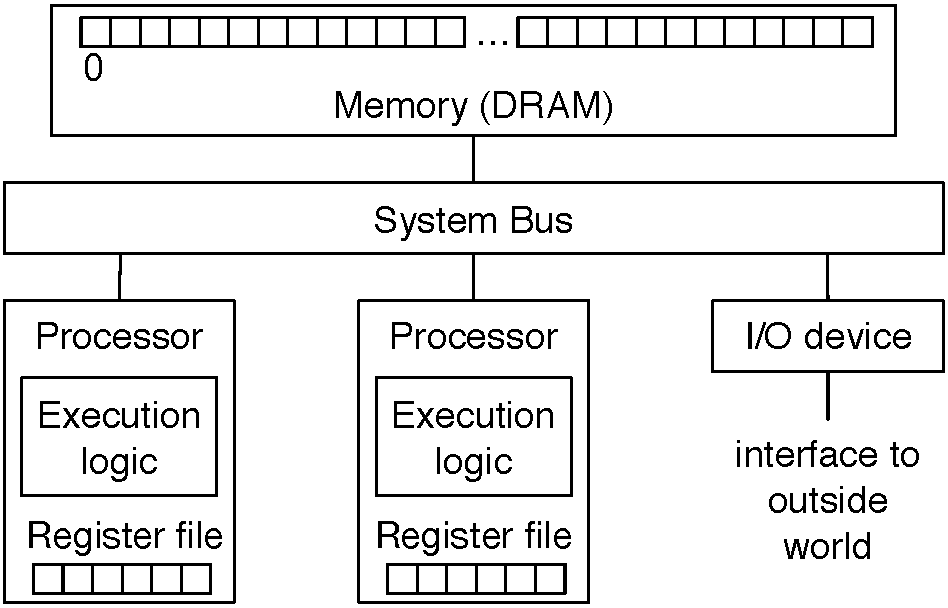
\includegraphics[width=65mm]{figures/computer_model.pdf}
  \caption{
    A computer's core is its processors and memory, which are connected by a
    system bus. Computers also have I/O devices, such as keyboards, which are
    also connected to the processor via the system bus.
  }
  \label{fig:computer_model}
\end{figure}


The building blocks for the model presented here come from
\cite{saltzer2009systemdesign}, which introduces the key abstractions in a
computer system, and  then focuses on the techniques used to build software
systems on top of these abstractions.

The memory is an array of storage cells, addressed using natural numbers
starting from 0, and implements the abstraction depicted in
Figure~\ref{fig:memory_abstraction}. Its salient feature is that the result of
reading a memory cell at an address must equal the most value written to that
memory cell.

\begin{figure}[hbt]
  \centering
  \begin{tabularx}{\columnwidth}{| X |}
  \hline
  \textsc{write}(\textit{addr}, \textit{value}) $ \rightarrow \varnothing $ \\
  Store \textit{value} in the storage cell identified by \textit{addr}. \\
  \hline
  \textsc{read}(\textit{addr}) $ \rightarrow $ \textit{value} \\
  Return the \textit{value} argument to the most recent \textsc{write} call
  referencing \textit{addr}. \\
  \hline
  \end{tabularx}
  \caption{The memory abstraction}
  \label{fig:memory_abstraction}
\end{figure}

A logical processor repeatedly reads \textit{instructions} from the
computer's memory and executes them, according to the flowchart in
Figure~\ref{fig:processor_execution}.

\begin{figure}[hbt]
  \centering
  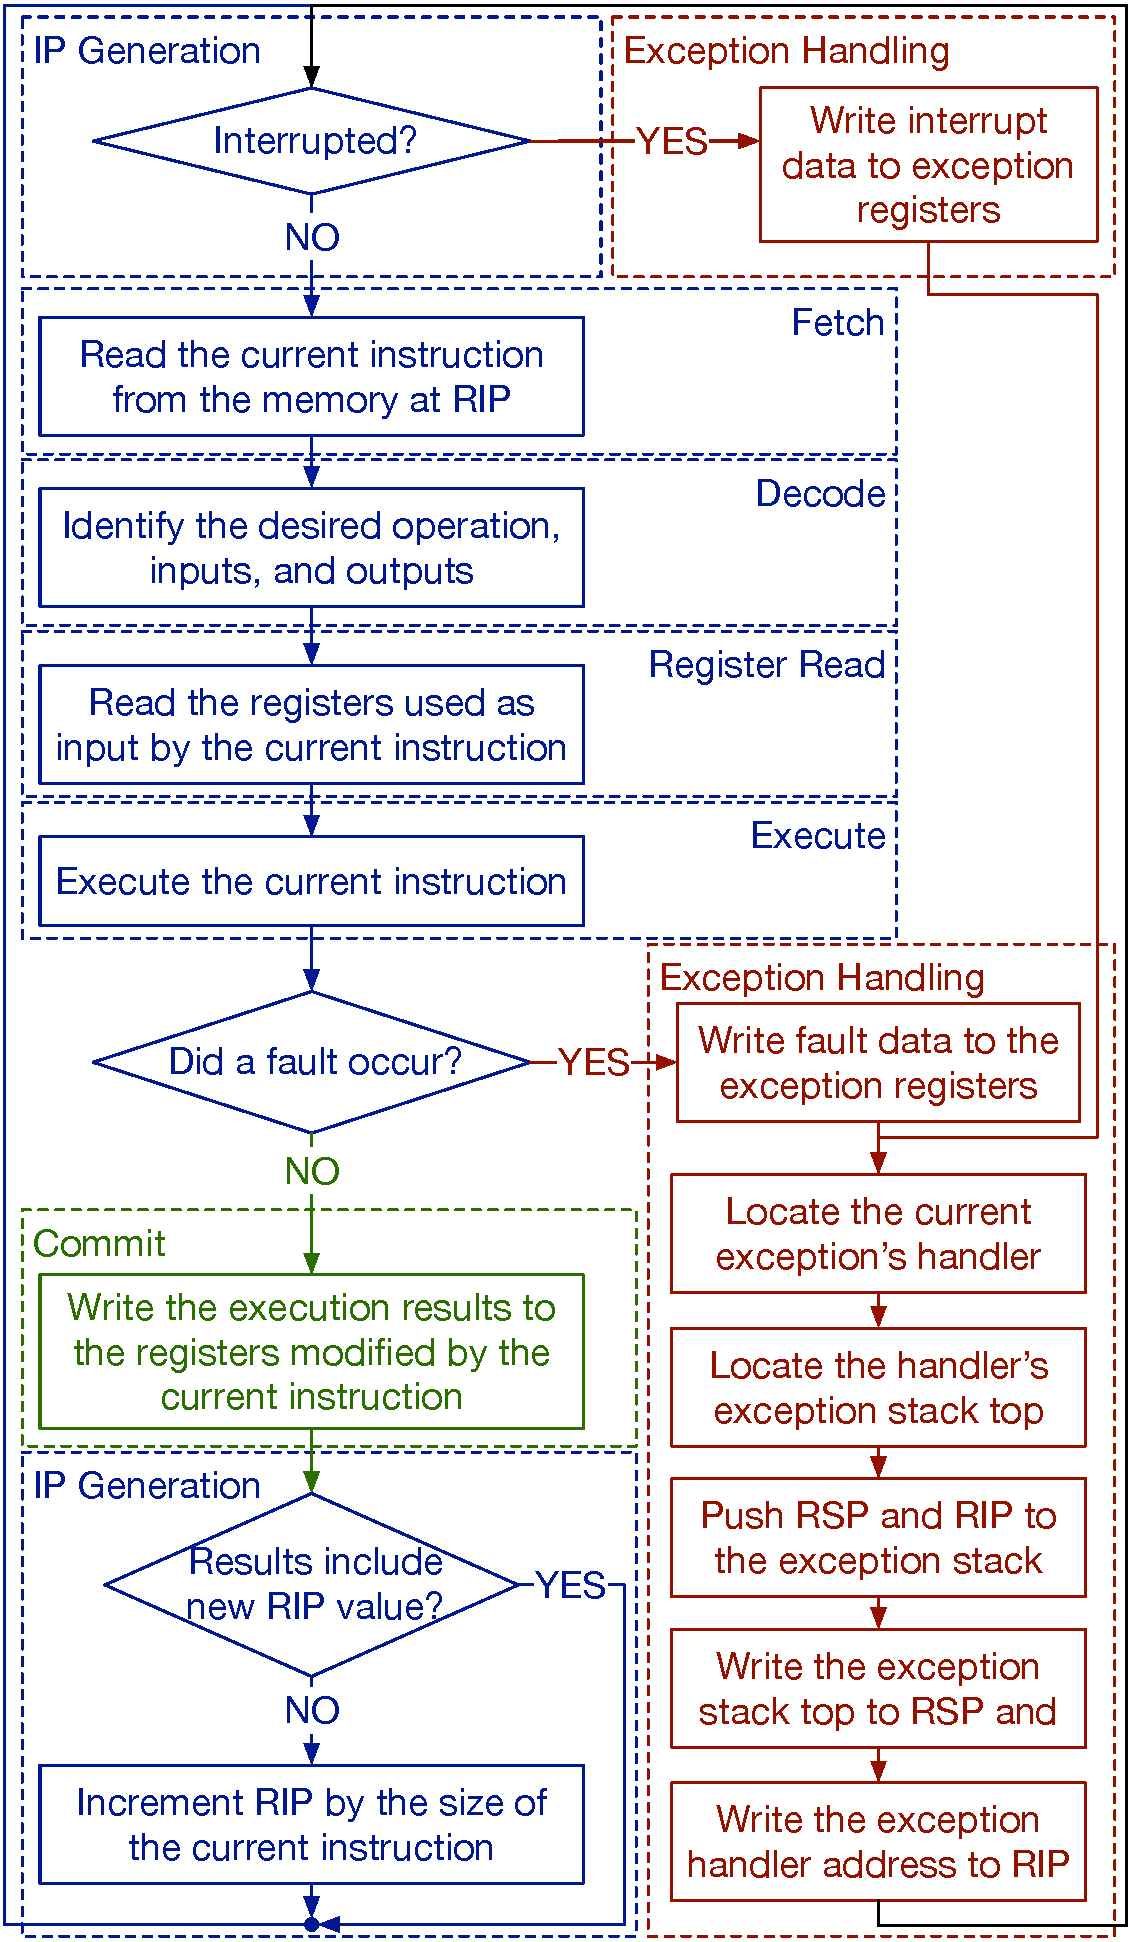
\includegraphics[width=85mm]{figures/processor_execution.pdf}
  \caption{
    A processor fetches instructions from the memory and executes them. The RIP
    register holds the address of the instruction to be executed.
  }
  \label{fig:processor_execution}
\end{figure}

The processor has an internal memory, referred to as the
\textit{register file}. The register file's memory cells, generally known as
\textit{registers}, make up the \textit{execution context} used to execute
instructions.

An instruction performs a simple computation on its inputs and stores the
result in an output location. For example, \texttt{ADD RDX, RAX, RBX} performs
an integer addition, where the inputs are the registers RAX and RBX, and the
result is stored in the output register RDX.

The registers mentioned in Figure~\ref{fig:processor_execution} are the
\textit{instruction pointer}~(RIP), which stores the memory  address of the
next instruction to be executed by the processor, and the
\textit{stack pointer}~(RSP), which stores the memory address of the topmost
element in the call stack used by the processor's procedural programming
support. The other execution context registers are described in
\S~\ref{sec:address_spaces} and \S~\ref{sec:registers}.

Under normal circumstances, the processor repeatedly reads an instruction from
the memory address stored in RIP, executes the instruction, and updates RIP to
point to the following instruction. Unlike many RISC architectures, the Intel
architecture uses a variable-size instruction encoding, so the size of an
instruction is not known until the instruction has been read from memory.

While executing an instruction, the processor may encounter a \textit{fault},
which is a situation where the instruction's preconditions are not met. When
a fault occurs, the instruction does not store a result in the output location.
Instead, the instruction's result is considered to be the fault that occurred.
For example, an integer division instruction \texttt{DIV} where the divisor is
zero results in a Division Fault (\#DIV).

When an instruction results in a fault, the processor stops its normal
execution flow, and performs the fault handler process documented in
\S~\ref{sec:faults}. In a nutshell, the processor first looks up the address of
the code that will handle the fault, based on the fault's nature, and sets up
the execution environment in preparation to execute the fault handler.

The processors are connected to each other and to the memory via a
\textit{system bus}, which is a broadcast network that implements the
abstraction in Figure~\ref{fig:bus_abstraction}.

\begin{figure}[hbt]
  \centering
  \begin{tabularx}{\columnwidth}{| X |}
  \hline
  \textsc{send}(\textit{op}, \textit{addr}, \textit{data})
  $ \rightarrow \varnothing $ \\
  Place a message containing the operation code \textit{op}, the bus address
  \textit{addr}, and the value \textit{data} on the bus. \\
  \hline
  \textsc{read}() $ \rightarrow $ (\textit{op}, \textit{addr},
  \textit{value}) \\
  Return the message that was written on the bus at the beginning of this
  clock cycle. \\
  \hline
  \end{tabularx}
  \caption{The system bus abstraction}
  \label{fig:bus_abstraction}
\end{figure}

During each clock cycle, at most one of the devices connected to the system bus
can send a message, which is received by all the other devices connected to the
bus. Each device attached to the bus decodes the operation codes and addresses
of all the messages sent on the bus and ignores the messages that do not
require its involvement.

For example, when the processor wishes to read a memory location, it sends a
message with the operation code \textsc{read-request} and the bus address
corresponding to the desired memory location. The memory sees the message on
the bus and performs the \textsc{read} operation. At a later time, the memory
responds by sending a message with the operation code \textsc{read-response},
the same address as the request, and the data value set to the result of the
\textsc{read} operation.

The computer communicates with the outside world via I/O devices, such as
keyboards, displays, and network cards, which are connected to the system bus.
Devices mostly respond to requests issued by the processor. However, devices
also have the ability to issue \textit{interrupt requests} that notify the
processor of outside events, such as the user pressing a key on a keyboard.

Interrupt triggering is discussed in \S~\ref{sec:interrupts}. On modern
systems, devices send interrupt requests by issuing writes to special bus
addresses. Interrupts are considered to be \textit{hardware exceptions}, just
like faults, and are handled in a similar manner.

\subsection{Software Privilege Levels}
\label{sec:rings}

In an Infrastructure-as-a-Service (IaaS) cloud environment, such as Amazon EC2,
commodity CPUs run software at four different privilege levels. The rest of the
section describes the privilege levels. We also point to successful exploits
that execute at each privilege level, motivating the SGX design decision to
assume that the host computer has malicious software running at all privilege
levels.

Figure~\ref{fig:cpu_rings} shows the privilege levels in the Intel
architecture. Software running at each level is strictly more powerful than
software running at less privileged levels. It follows that software running at
a level can access the code and data at less privileged levels, and compromise
the software running at these levels. Thus, software at each level must trust
all the software running at more privileged levels.

\begin{figure}[hbtp]
  \centering
  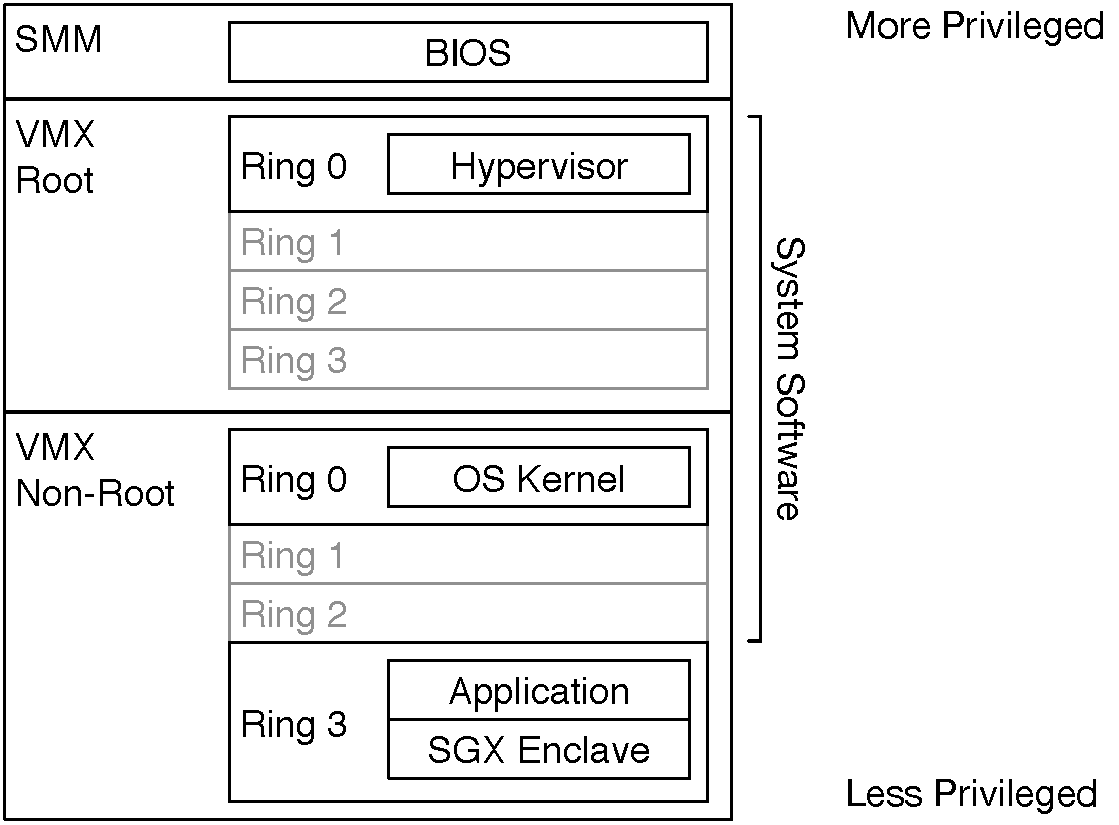
\includegraphics[width=85mm]{figures/cpu_rings.pdf}
  \caption{
    The privilege levels in the x86 architecture, and the software that
    typically runs at each security level.
  }
  \label{fig:cpu_rings}
\end{figure}

% System Management Mode: SDM S 34

\textit{System Management Mode} (SMM) is intended for use by the motherboard
manufacturers to implement features such as fan control and deep sleep, and/or
to emulate missing hardware. SMM mode is entered by sending the CPU an SMI
signal, which was initially designed exclusively for hardware use, and only
produced when the SMI\# pin was asserted on the CPU's chip package. However, in
modern systems, system software can generate an SMI, using the methods in
\S~\ref{sec:interrupts}. This opens up the avenue for SMM-based software
exploits.

The SMM code and data are stored in a contiguous subset of DRAM called
\textit{System Management RAM} (SMRAM) which, in theory, is not readable or
writable when the processor isn't running in SMM. However, its protection
mechanisms were bypassed multiple times~\cite{duflot2006smm,
rutkowska2008remap, wojtczuk2009smm, kallenberg2014smm}, and SMM-based
rootkits~\cite{wecherowski2009smm, embleton2010smm} have been demonstrated.

IaaS cloud providers allow their customers to run their operating system of
choice in a virtualized environment. Hardware
virtualization~\cite{uhlig2005vmx}, called \textit{Virtual Machine Extensions}
(VMX) by Intel, adds support for a \textit{hypervisor}, also called a
Virtual Machine Monitor (VMM) in the Intel documentation. The hypervisor runs
at a higher privilege level (VMX root mode) than the operating system, and is
responsible for allocating hardware resources across multiple operating systems
that share the same physical machine. The hypervisor uses the CPU's hardware
virtualization features to make each operating system believe it is running in
its own computer, called a \textit{virtual machine} (VM). Hypervisor code
generally runs at ring 0 in VMX root mode.

The popular Xen hypervisor uses VMX root mode to obtain better peformance and a
smaller codebase \cite{zhang2008xen} than virtualization software based on
binary translation \cite{rosenblum2005virtualization}. Despite its relatively
small codebase, Xen has had over 40 security vulnerabilities patched in
\textbf{each} of the last three years (2012-2014) \cite{cvedetails2014xen}.

\cite{mccune2010trustvisor} proposes using a very small hypervisor together
with Intel TXT's dynamic root of trust for measurement (DRTM) to implement
trusted execution. \cite{vasudevan2010requirements} argues that a dynamic root
of trust mechanism, like Intel TXT, is necessary to ensure a hypervisor's
integrity.  Unfortunately, the TXT design requires an implementation complex
enough that security vulnerabilities have been found \cite{wojtczuk2009txt2}
\cite{wojtczuk2011txt}. Furthermore, any SMM attack can be used to compromise
TXT \cite{wojtczuk2009txt}.

The systems research literature recommends breaking up an operating system into
a small \textit{kernel}, which runs at a high privilege level, known as the
\textit{kernel mode} or \textit{supervisor mode} and, in the Intel
architecture, as \textit{ring 0}. The kernel allocates the computer's resources
to the other system components, such as device drivers and services, which run
at lower privilege levels. However, for performance reasons\footnote{Switching
between rings is much slower than a normal procedure call.}, mainstream
operating systems have large amounts of code running at ring 0. Their
\textit{monolithic kernels} include device drivers, filesystem code, networking
stacks, and video rendering functionality.

The monolithic kernel design leads to many opportunities for security
vulnerabilities in kernel code. For example the Linux kernel has had over 100
security vulnerabilities patched in \textbf{each} of the last three years
(2012-2014) \cite{cvedetails2014linux} \cite{chen2011linux}. Also, a successful
attack on SMM or the hypervisor trivially translates into a compromised kernel.

Application code, such as a Web server or a game client, runs at the lowest
privilege level, referred to as \textit{user mode} (\textit{ring 3} in the
Intel architecture). In IaaS cloud environments, the virtual machine images
provided by customers run in VMX non-root mode, so the kernel runs in VMX
non-root ring 0, and the application code runs in VMX non-root ring 3.

\subsection{Address Spaces}
\label{sec:address_spaces}

While performing computation, a commodity Intel CPU moves data between four
distinct physical address spaces, shown in Figure~\ref{fig:address_spaces}. The
address spaces overlap partially, in both purpose and contents, which can lead
to confusion. This section gives a high-level overview of the physical address
spaces defined by the Intel architecture, with an emphasis on their purpose and
the methods used to manage them.

\begin{figure}[hbtp]
  \center{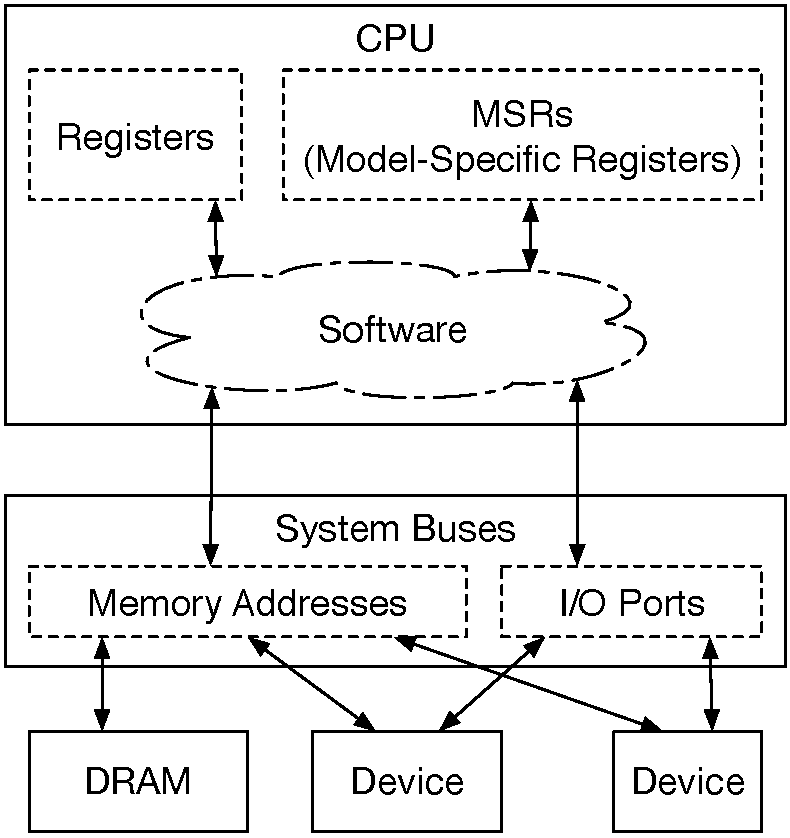
\includegraphics[width=55mm]{figures/address_spaces.pdf}}
  \caption{
    The four physical address spaces used by an Intel CPU. The registers and
    MSRs are internal to the CPU, while the memory and I/O address spaces are
    used to communicate with DRAM and other devices via system buses.
  }
  \label{fig:address_spaces}
\end{figure}

The \textit{register} space consists of names that are used to access the CPU's
register file, which is the only memory that operates at the CPU's clock
frequency and can be used without any latency penalty. The register space is
defined by the CPU's architecture, and documented in the SDM.

Some registers, such as the \textit{Control Registers} (CRs) play specific
roles in configuring the CPU's operation. For example, CR3 plays a central role
in address translation (\S~\ref{sec:paging}). These registers can only be
accessed by system software. The rest of the registers make up an application's
\textit{execution context} (\S~\ref{sec:registers}), which is essentially a
high-speed scratch space. These registers can by accessed at all privilege
levels, and their allocation is managed by the software's compiler. Many CPU
instructions only operate on data in registers, and only place their results in
registers.

The \textit{memory} space, generally referred to as \textit{the address space}
\textit{the physical address space}, consists of $2^{36}$ (64 GB) - $2^{40}$
(1 TB) addresses. The memory space is primarily used to access
\textit{Dynamic Random-Access Memory} (DRAM), the computer's main memory, but
it is also used to communicate with \textit{memory-mapped devices} that read
memory requests off a system bus and write replies for the CPU. Some CPU
instructions can read their inputs from the memory space, or store the results
using the memory space.

A better-known example of memory mapping is that at computer startup, memory
addresses 0xFFFFF000 - 0xFFFFFFFF (the 64 KB of memory right below the 4 GB
mark) are mapped to a flash memory device that holds the code for booting the
computer.

This memory space is partitioned between devices and DRAM by the computer's
firmware during the boot stage. Sometimes, system software includes
motherboard-specific code that modifies the memory space partitioning. The OS
kernel relies on address translation, described in \S~\ref{sec:paging}, to
control the applications' access to the memory space. The hypervisor relies on
the same mechanism to control the guest OSes.

% I/O Address Space: SDM vol1 S 16.3

The \textit{input/output} (I/O) space consists of $2^{16}$ I/O addresses,
usually called \textit{ports}. The I/O ports are used exclusively to
communicate with devices. The CPU provides specific instructions for reading
from and writing to the I/O space. I/O ports are allocated to devices by formal
or de-facto standards. For example, ports 0xCF8 and 0xCFC are always used to
access the PCI express (\S~\ref{sec:motherboard}) configuration space.

The CPU implements a mechanism for system software to provide fine-grained I/O
access to applications. However, all modern kernels restrict application
software from accessing the I/O space directly, in order to limit the damage
potential of application bugs.

% Architectural MSRs: SDM S 35.1
% Time-Stamp Counter: SDM S 17.13

The \textit{Model-Specific Register} (MSR) space consists of $2^{32}$ MSRs,
which are used to configure the CPU's operation. The MSR space was initially
intended for the use of CPU model-specific firmware, but some MSRs have been
promoted to \textit{architectural MSR} status, making their semantics a part of
the Intel architecture. For example, architectural MSR 0x10 holds a
high-resolution monotonically increasing time-stamp counter.

The CPU provides instructions for reading from and writing to the MSR space.
The instructions can only be used by system software. Some MSRs are also
exposed by instructions accessible to applications. For example, applications
can read the time-stamp counter with the \texttt{RDTSC} and \texttt{RDTSCP},
which are very useful for benchmarking and optimizing software, but also for
mounting timing attacks.

\HeadingLevelB{Address Translation}
\label{sec:paging}

% Outcome: understanding the isolation provided by address translation

System software relies on the CPU's address translation mechanism for
implementing isolation among less privileged pieces of software (applications
or operating systems). Virtually all secure architecture designs bring changes
to address translation. We summarize the Intel architecture's address
translation features that are most relevant when establishing a system's
security properties, and refer the reader to \cite{jacob1998virtual} for a more
general presentation of address translation concepts and its other uses.


\HeadingLevelC{Address Translation Concepts}
\label{sec:paging_concepts}
\label{sec:paging_vpn}
\label{sec:paging_ppn}

From a systems perspective, address translation is a layer of indirection
(shown in Figure~\ref{fig:address_translation}) between the
\textit{virtual addresses}, which are used by a program's memory load and store
instructions, and the \textit{physical addresses}, which reference the physical
address space (\S~\ref{sec:address_spaces}). The mapping between virtual and
physical addresses is defined by \textit{page tables}, which are managed by the
system software.

\begin{figure}[hbt]
  \centering
  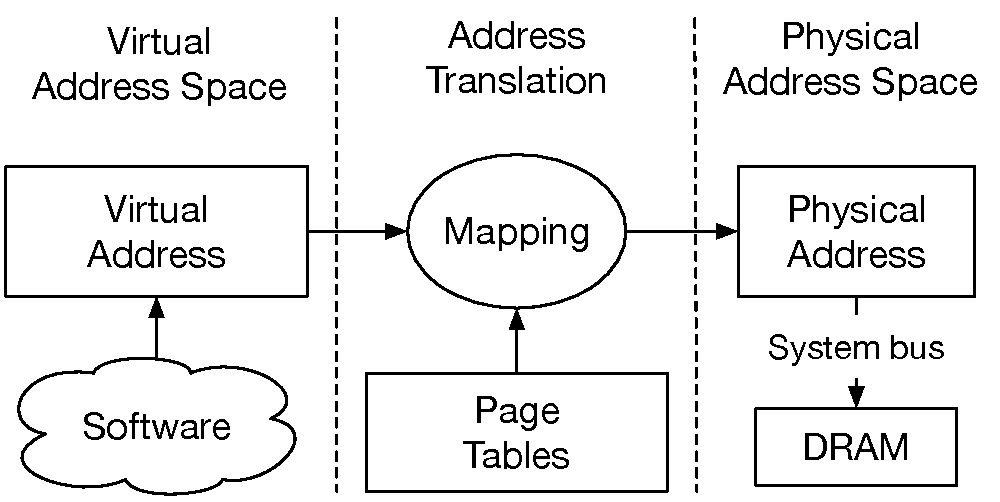
\includegraphics[width=75mm]{figures/address_translation.pdf}
  \caption{
    Virtual addresses used by software are translated into physical memory
    addresses using a mapping defined by the page tables.
  }
  \label{fig:address_translation}
\end{figure}

Operating systems use address translation to implement the \textit{virtual
memory abstraction}, illustrated by Figure~\ref{fig:virtual_memory}. The
virtual memory abstraction exposes the same interface as the memory abstraction
in \S~\ref{sec:resources}, but each process uses a separate virtual address
space that only references the memory allocated to that process. From an
application developer standpoint, virtual memory can be modeled by pretending
that each process runs on a separate computer and has its own DRAM.

\begin{figure}[hbt]
  \centering
  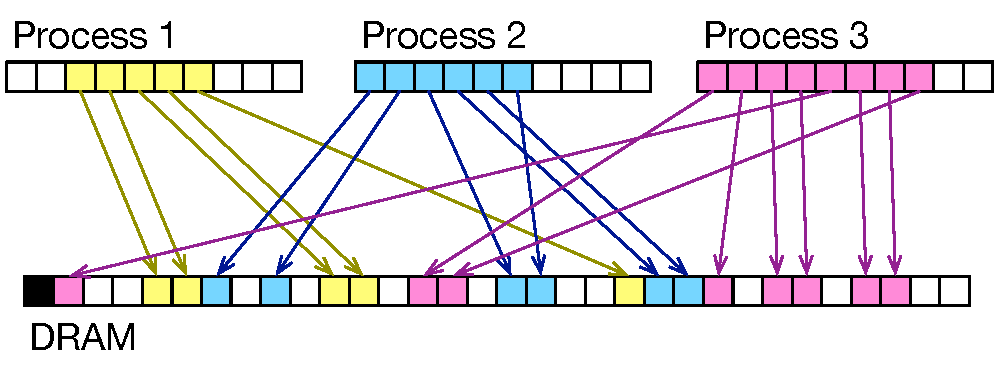
\includegraphics[width=80mm]{figures/virtual_memory.pdf}
  \caption{
    The virtual memory abstraction gives each process its own virtual address
    space. The operating system multiplexes the computer's DRAM between the
    processes, while application developers build software as if it owns the
    entire computer's memory.
  }
  \label{fig:virtual_memory}
\end{figure}

Address translation is used by the operating system to multiplex DRAM among
multiple application processes, isolate the processes from each other, and
prevent application code from accessing memory-mapped devices directly. The
latter two protection measures prevent an application's bugs from impacting
other applications or the OS kernel itself. Hypervisors also use address
translation, to divide the DRAM among operating systems that run concurrently,
and to virtualize memory-mapped devices.

% Canonical Addressing: SDM vol1 S 3.3.7.1
% IA-32e Paging: SDM S 4.5

The address translation mode used by 64-bit operating systems, called
IA-32e by Intel's documentation, maps 48-bit \textit{virtual addresses} to
\textit{physical addresses} of at most 52 bits\footnote{The size of a
physical address is CPU-dependent, and is 40 bits for recent desktop CPUs and
44 bits for recent high-end server CPUs.}. The translation process, illustrated
in Figure~\ref{fig:os_paging}, is carried out by dedicated hardware in the CPU,
which is referred to as the \textit{address translation unit} or the
\textit{memory management unit} (MMU).

\begin{figure}[hbt]
  \centering
  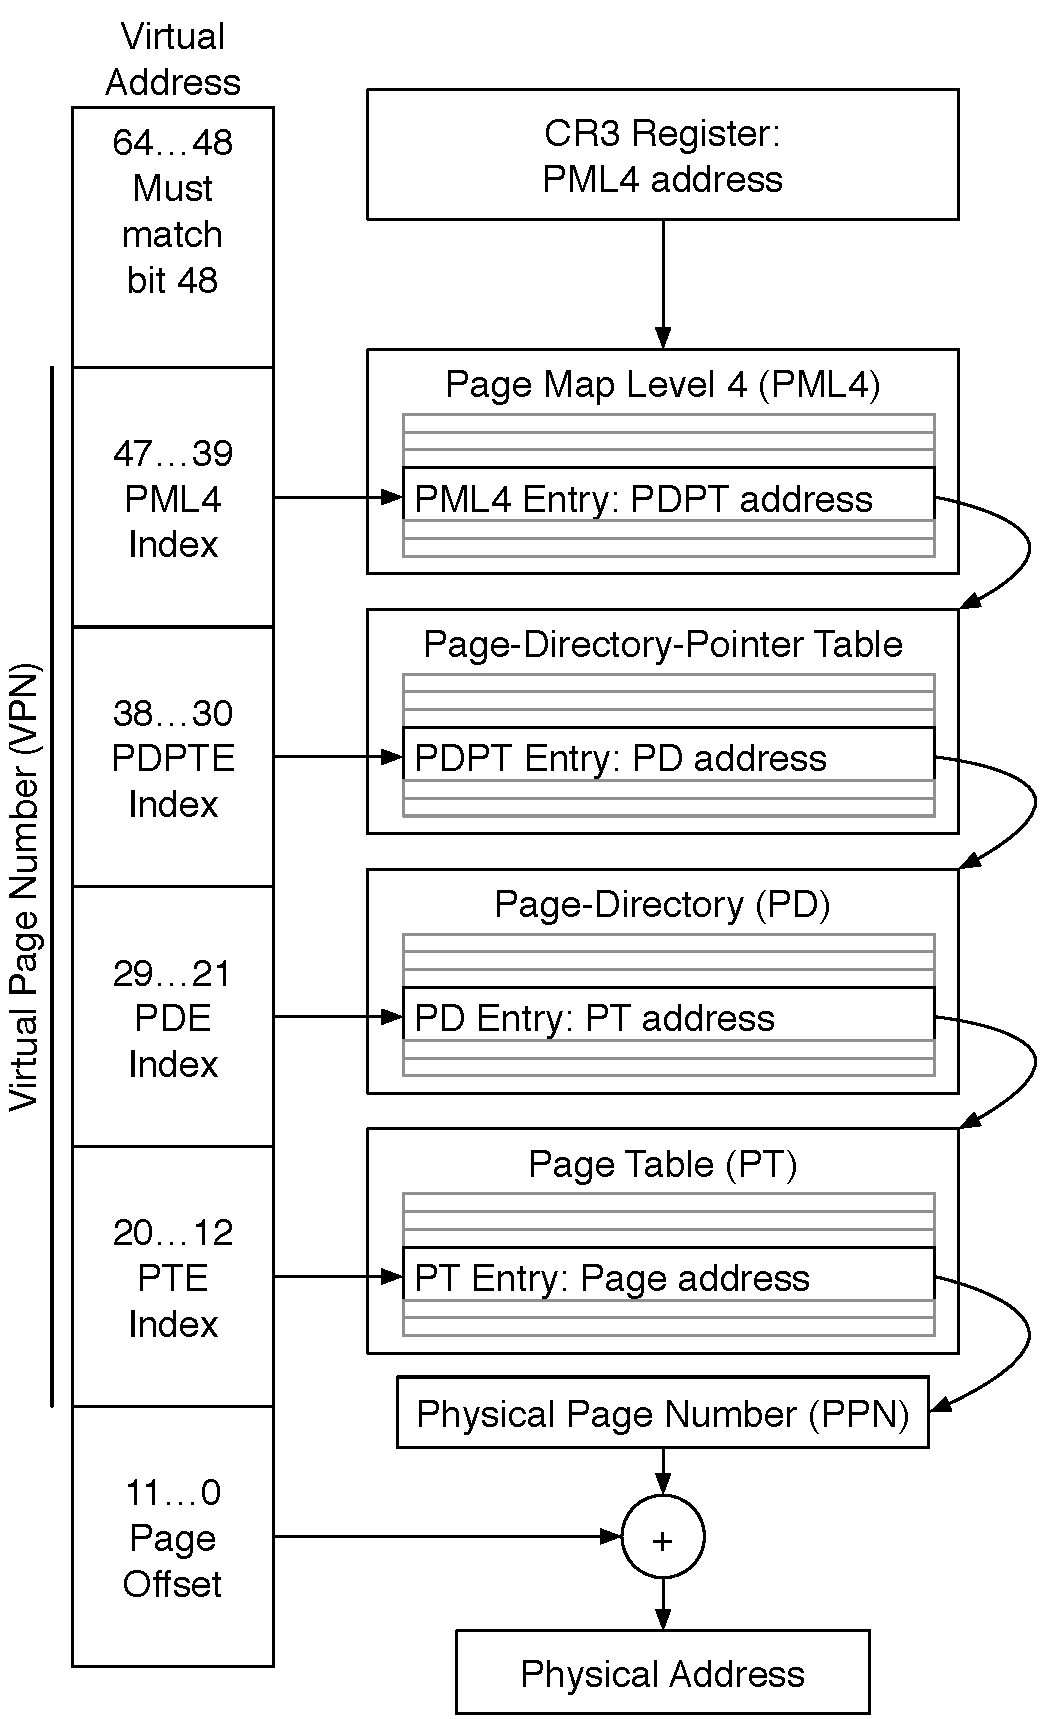
\includegraphics[width=80mm]{figures/os_paging.pdf}
  \caption{
    IA-32e address translation takes in a 48-bit virtual address and outputs
    a 52-bit physical address.
  }
  \label{fig:os_paging}
\end{figure}

The bottom 12 bits of a virtual address are not changed by the translation. The
top 36 bits are grouped into four 9-bit indexes, which are used to index into
the page tables. Despite its name, the page tables data structure closely
resembles a full 512-ary search tree where nodes have fixed keys. Each
node is represented in DRAM as an array of 512 8-byte entries that contain the
physical addresses of the next-level children as well as some flags. The
physical address of the root node is stored in the CR3 register. The arrays in
the last-level nodes contain the physical addresses that are the result of the
address translation.

The address translation function, which does not change the bottom bits of
addresses, partitions the memory address space into \textit{pages}. A page is
the set of all memory locations that only differ in the bottom bits which are
not impacted by address translation, so all the memory addresses in a virtual
page translate to corresponding addresses in the same physical page. From this
perspective, the address translation function can be seen as a mapping between
\textit{Virtual Page Numbers} (VPN) and \textit{Physical Page Numbers} (PPN),
as shown in Figure~\ref{fig:address_translation_bits}.

\begin{figure}[hbt]
  \centering
  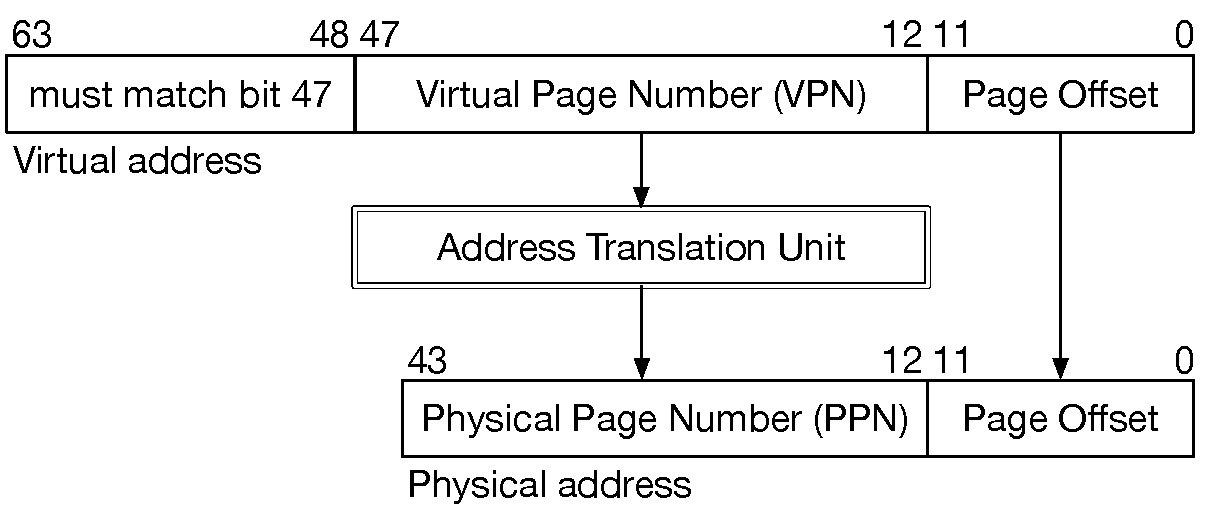
\includegraphics[width=85mm]{figures/address_translation_bits.pdf}
  \caption{
    Address translation can be seen as a mapping between virtual page numbers
    and physical page numbers.
  }
  \label{fig:address_translation_bits}
\end{figure}

In addition to isolating application processes, operating systems also use the
address translation feature to run applications whose collective memory
demands exceed the amount of DRAM installed in the computer. The OS evicts
infrequently used memory pages from DRAM to a larger (but slower) memory, such
as a hard disk drive (HDD) or solid-state drive (SSD). For historical reason,
this slower memory is referred to as the \textit{disk}.

The OS ability to over-commit DRAM is often called \textit{page swapping}, for
the following reason. When an application process attempts to access a page
that has been evicted, the OS ``steps in'' and reads the missing page back into
DRAM. In order to do this, the OS might have to evict a different page from
DRAM, effectively swapping the contents of a DRAM page with a disk page. The
details behind this high-level description are covered in the following
sections.

The CPU's address translation is also referred to as ``paging'', which is a
shorthand for ``page swapping''.


\HeadingLevelC{Address Translation and Virtualization}
\label{sec:vmx_paging}

% VMX Support for Address Translation: SDM S 4.11

Computers that take advantage of hardware virtualization use a hypervisor to
run multiple operating systems at the same time. This creates some tension,
because each operating system was written under the assumption that it owns the
entire computer's DRAM. The tension is solved by a second layer of address
translation, illustrated in Figure~\ref{fig:vmx_address_translation}.

\begin{figure}[hbt]
  \centering
  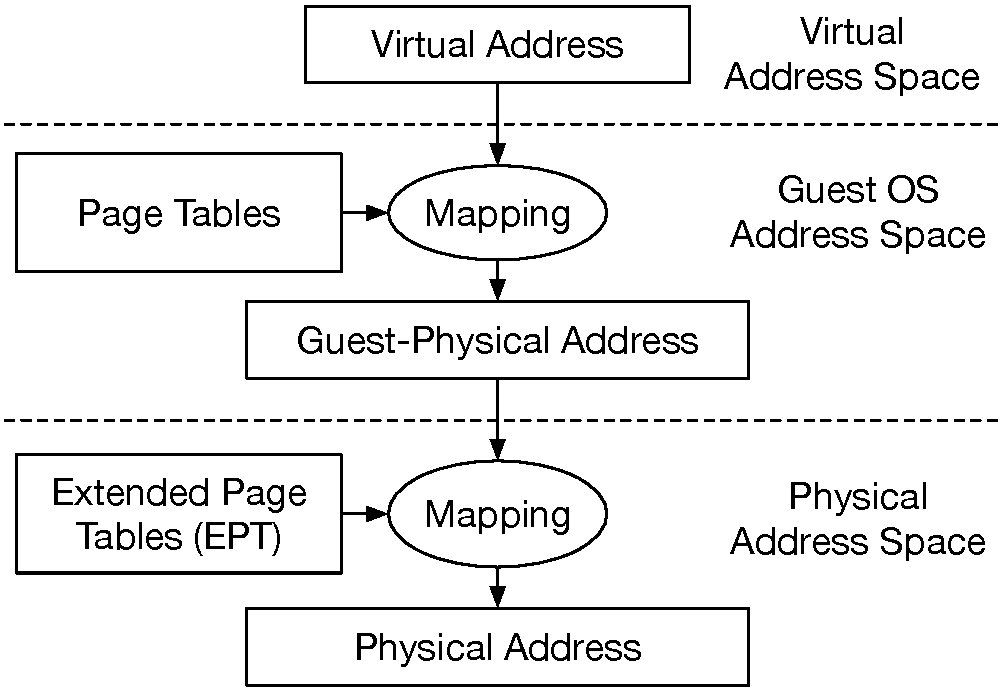
\includegraphics[width=70mm]{figures/vmx_address_translation.pdf}
  \caption{
    Virtual addresses used by software are translated into physical memory
    addresses using a mapping defined by the page tables.
  }
  \label{fig:vmx_address_translation}
\end{figure}


When a hypervisor is active, the page tables set up by an operating system map
between virtual addresses and \textit{guest-physical addresses} in a
\textit{guest-physical address space}. The hypervisor multiplexes the
computer's DRAM between the operating systems' guest-physical address spaces
via the second layer of address translations, which uses \textit{extended page
tables}~(EPT) to map guest-physical addresses to physical addresses.

The EPT uses the same data structure as the page tables, so the process of
translating guest-physical addresses to physical addresses follows the same
steps as IA-32e address translation. The main difference is that the physical
address of the data structure's root node is stored in the extended page table
pointer~(EPTP) field in the \textit{Virtual Machine Control Structure}~(VMCS)
for the guest OS. Figure~\ref{fig:vmx_paging} illustrates the address
translation process in the presence of hardware virtualization.

\begin{figure}[hbt]
  \centering
  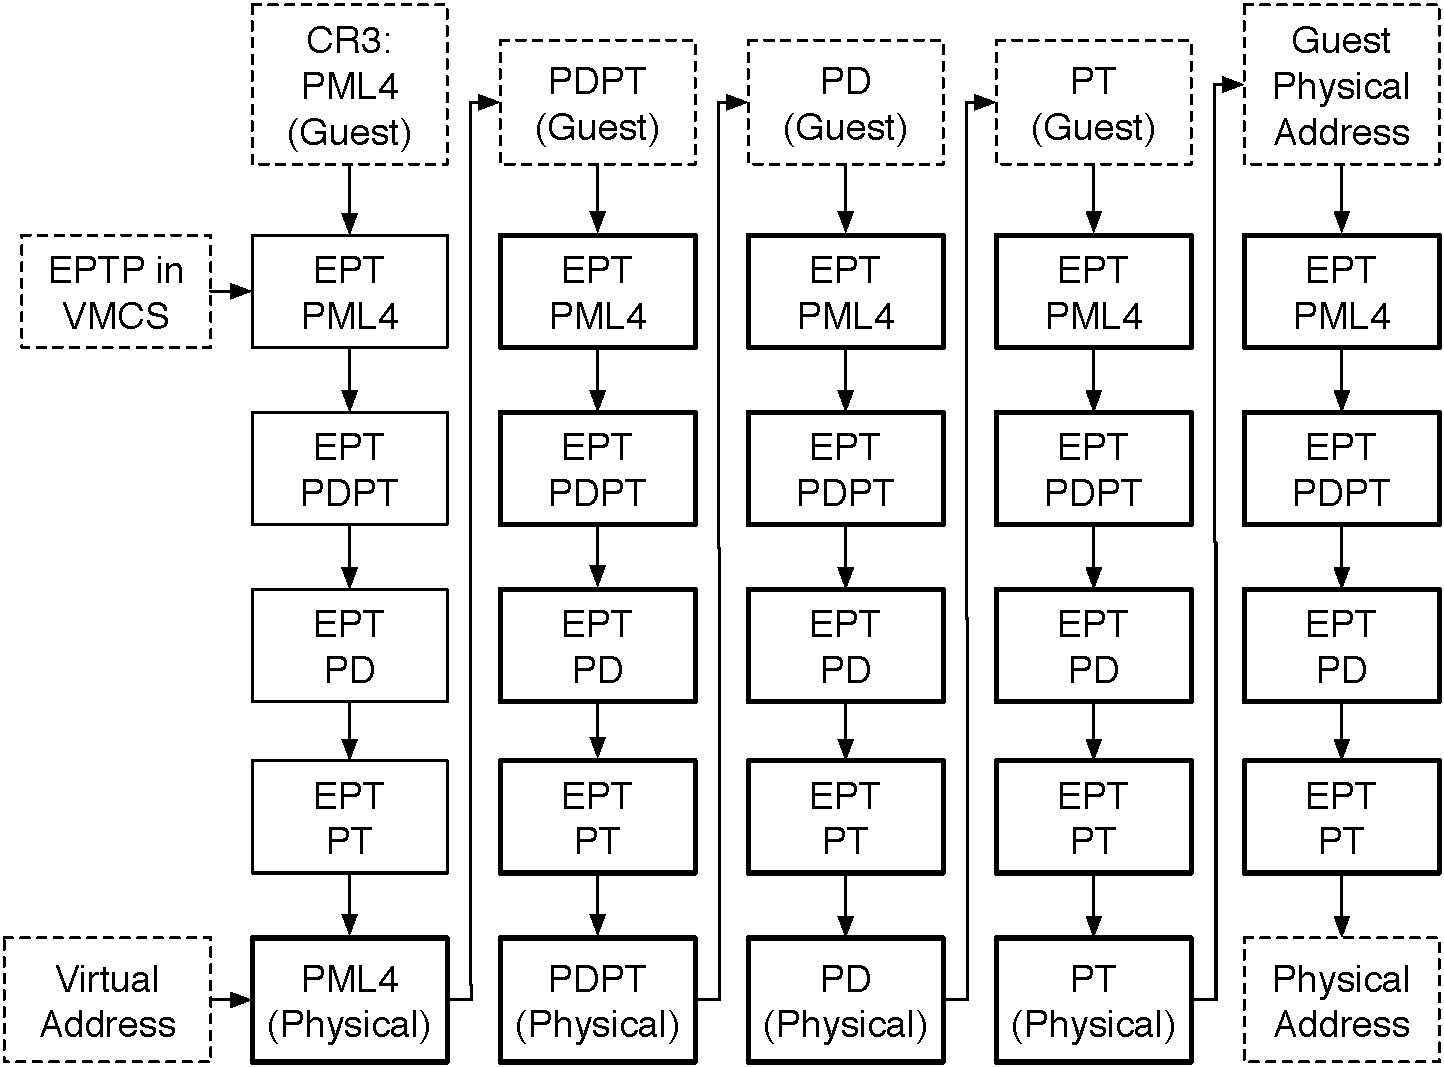
\includegraphics[width=85mm]{figures/vmx_paging.pdf}
  \caption{
    Address translation when hardware virtualization is enabled. The
    kernel-managed page tables contain guest-physical addresses, so each level
    in the kernel's page table requires a full walk of the hypervisor's
    extended page table~(EPT).  A translation requires up to 20 memory accesses
    (the bold boxes), assuming the physical address of the kernel's PML4 is
    cached.
  }
  \label{fig:vmx_paging}
\end{figure}


\HeadingLevelC{Page Table Attributes}
\label{sec:page_table_attributes}

Each page table entry contains a physical address, as shown in
Figure~\ref{fig:os_paging}, and some Boolean values that are referred to as
\textit{flags} or \textit{attributes}. The following attributes are used to
implement page swapping and software isolation.

The \textit{present}~(P) flag is set to 0 to indicate unused parts
of the address space, which do not have physical memory associated with them.
The system software also sets the P flag to 0 for pages that are evicted from
DRAM. When the address translation unit encounters a zero P flag, it aborts the
translation process and issues a hardware exception, as described in
\S~\ref{sec:faults}. This hardware exception gives system software an
opportunity to step in and bring an evicted page back into DRAM.

The \textit{accessed}~(A) flag is set to 1 by the CPU whenever the address
translation machinery reads a page table entry, and the \textit{dirty}~(D) flag
is set to 1 by the CPU when an entry is accessed by a memory write operation.
The A and D flags give the hypervisor and kernel insight into application
memory access patterns and inform the algorithms that select the pages that get
evicted from RAM.

% Page-Level Protection: SDM S 5.11, S 5.11.{1,2,3,4}

The main attributes supporting software isolation are the
\textit{writable}~(W) flag, which can be set to 0 to
prohibit\footnote{Writes to non-writable pages result in \#GP exceptions
(\S~\ref{sec:faults}).} writes to any memory location inside a page, the
\textit{disable execution}~(XD) flag, which can be set to 1 to prevent
instruction fetches from a page, and the \textit{supervisor}~(S) flag, which
can be set to 1 to prohibit any accesses from application software running at
ring 3.

\HeadingLevelB{Execution Contexts}
\label{sec:registers}

Application software targeting the 64-bit Intel architecture uses a variety of
CPU registers to interact with the processor's features, shown in
Figure~\ref{fig:cpu_registers} and Table~\ref{fig:xsave_state}. The values in
these registers make up an application thread's state, or \textit{execution
context}.

OS kernels multiplex each logical processor (\S~\ref{sec:cpu_core}) between
multiple software threads by \textit{context switching}, namely saving the
values of the registers that make up a thread's execution context, and
replacing them with another thread's previously saved context. Context
switching also plays a part in executing code inside secure containers, so its
design has security implications.

% 64-Bit Mode Execution Environment: SDM vol1 S 3.2.1
% Basic Program Execution Registers: SDM vol1 S 3.4

\begin{figure}[hbt]
  \centering
  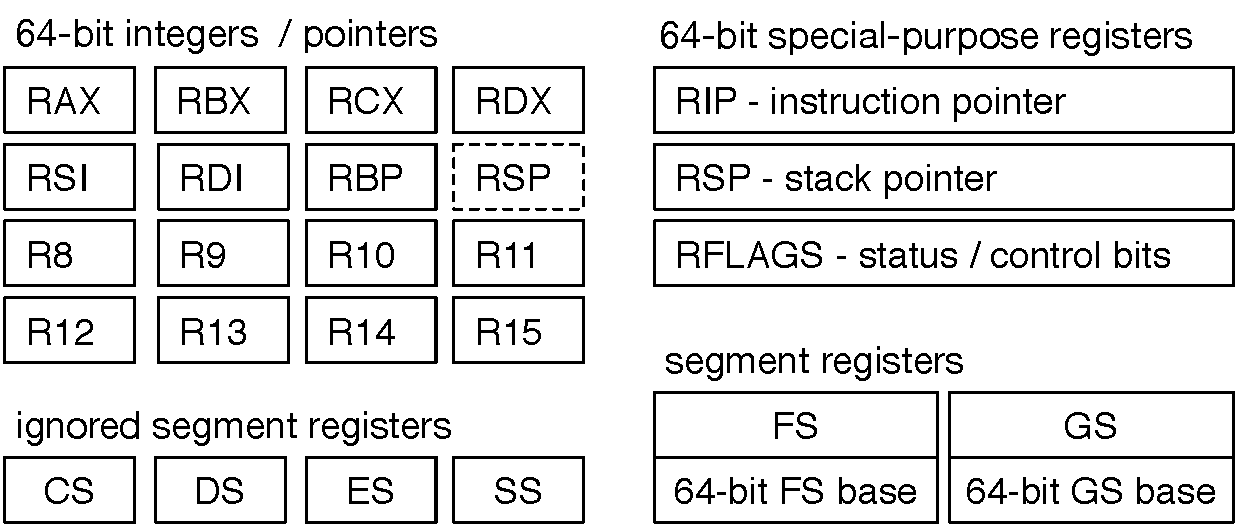
\includegraphics[width=85mm]{figures/cpu_registers.pdf}
  \caption{
    CPU registers in the 64-bit Intel architecture. RSP can be used as a
    general-purpose register (GPR), e.g., in pointer arithmetic, but it always
    points to the top of the program's stack. Segment registers are covered in
    \S~\ref{sec:segments}.
  }
  \label{fig:cpu_registers}
\end{figure}

Integers and memory addresses are stored in 16 \textit{general-purpose
registers} (GPRs). The first 8 GPRs have historical names: RAX, RBX, RCX,
RDX, RSI, RDI, RSP, and RBP, because they are extended versions of the 32-bit
Intel architecture's GPRs. The other 8 GPRs are simply known as R9-R16. RSP is
designated for pointing to the top of the procedure call stack, which is simply
referred to as \textit{the stack}. RSP and the stack that it refers to are
automatically read and modified by the CPU instructions that implement
procedure calls, such as \texttt{CALL} and \texttt{RET} (return), and by
specialized stack handling instructions such as \texttt{PUSH} and \texttt{POP}.

All applications also use the RIP register, which contains the address of the
currently executing instruction, and the RFLAGS register, whose bits (e.g.,
the carry flag - CF) are individually used to store comparison results and
control various instructions.

% XSAVE-Supported Features and State-Component Bitmaps: SDM vol1 S 13.1
% Enabling the XSAVE Feature Set and XSAVE-Enabled Features: SDM vol1 S13.3
% XSAVE-managed State: SDM vol1 S 13.5

Software might use other registers to interact with specific processor
features, some of which are shown in Table~\ref{fig:xsave_state}.

\begin{table}[hbt]
  \centering
  \begin{tabularx}{\columnwidth}{| l | X | l |}
  \hline
  \textbf{Feature} & \textbf{Registers} & \textbf{XCR0 bit}\\
  \hline
  FPU & FP0 - FP7, FSW, FTW & 0 \\
  \hline
  SSE & MM0 - MM7, XMM0 - XMM15, XMCSR & 1 \\
  \hline
  AVX & YMM0 - YMM15 & 2 \\
  \hline
  MPX & BND0 - BND 3 & 3 \\
  \hline
  MPX & BNDCFGU, BNDSTATUS & 4 \\
  \hline
  AVX-512 & K0 - K7 & 5 \\
  \hline
  AVX-512 & ZMM0\_H  - ZMM15\_H & 6 \\
  \hline
  AVX-512 & ZMM16 - ZMM31 & 7 \\
  \hline
  PK & PKRU & 9 \\
  \hline
  \end{tabularx}
  \caption{Sample feature-specific Intel architecture registers.}
  \label{fig:xsave_state}
\end{table}

The Intel architecture provides a future-proof method for an OS kernel to save
the values of feature-specific registers used by an application. The
\texttt{XSAVE} instruction takes in a \textit{requested-feature bitmap}~(RFBM),
and writes the registers used by the features whose RFBM bits are set to 1 in a
memory area. The memory area written by \texttt{XSAVE} can later be used by the
\texttt{XRSTOR} instruction to load the saved values back into feature-specific
registers. The memory area includes the RFBM given to \texttt{XSAVE}, so
\texttt{XRSTOR} does not require an RFBM input.

Application software declares the features that it plans to use to the kernel,
so the kernel knows what XSAVE bitmap to use when context-switching. When
receiving the system call, the kernel sets the XCR0 register to the feature
bitmap declared by the application. The CPU generates a fault if application
software attempts to use features that are not enabled by XCR0, so applications
cannot modify feature-specific registers that the kernel wouldn't take into
account when context-switching. The kernel can use the \texttt{CPUID}
instruction to learn the size of the \texttt{XSAVE} memory area for a given
feature bitmap, and compute how much memory it needs to allocate for the
context of each of the application's threads.

\subsection{Segment Registers}
\label{sec:segments}

The price of the Intel 64-bit architecture's widespread adoption was the
ability to run software targeting the older 32-bit architecture side-by-side
with 64-bit software \cite{cnet2005itanium}, which resulted in some warts in
the 64-bit architecture. While most warts are not material to the understanding
and operation of SGX, the 64-bit architecture's segment registers and vestigial
segmentation model must be understood. Therefore, this section covers the
segmentation concepts needed to understand SGX.

The semantics of the Intel architecture's instructions include the implicit use
of a few segments which are loaded into the processor's
\textit{segment registers} shown in Figure~\ref{fig:cpu_registers}. Code
fetches use the \textit{code segment} (CS).  Instructions that reference the
stack implicitly use the \textit{stack segment} (SS). Memory references
implicitly use the \textit{data segment} (DS) or the \textit{destination
segment} (ES). Via segment override prefixes, instructions can be modified to
use the unnamed segments FS and GS for memory references.

Modern operating systems effectively disable segmentation by covering the
entire addressable space with one segment, which is loaded in CS, and one data
segment, which is loaded in SS, DS and ES. The FS and GS registers store
segments covering \textit{thread-local storage} (TLS).

% Segment Selectors: SDM S 3.4.2
% Segment Registers: SDM S 3.4.3

Due to the Intel architecture's 16-bit origins, segment registers are exposed
as 16-bit values, called \textit{segment selectors}. The top 13 bits in a
selector are an index in a \textit{descriptor table}, and the bottom 2 bits are
the selector's ring number, which is also called requested privilege level
(RPL) in the Intel documentation. Also, modern system software only uses rings
0 and 3 (see \S~\ref{sec:rings}).

% Segment Loading Instructions in IA-32e Mode: SDM S 3.4.4
% Limit Checking in 64-bit Mode: SDM S 5.3.1
% Privilege Levels: SDM S 5.5

Each segment register has a hidden \textit{segment descriptor}, which consists
of a \textit{base address}, \textit{limit}, and type information, such as
whether the descriptor should be used for executable code or data.
Figure~\ref{fig:cpu_segment} shows the effect of loading a 16-bit selector into
a segment register. The selector's index is used to read a descriptor from the
descriptor table and copy it into the segment register's hidden descriptor.

\begin{figure}[hbt]
  \center{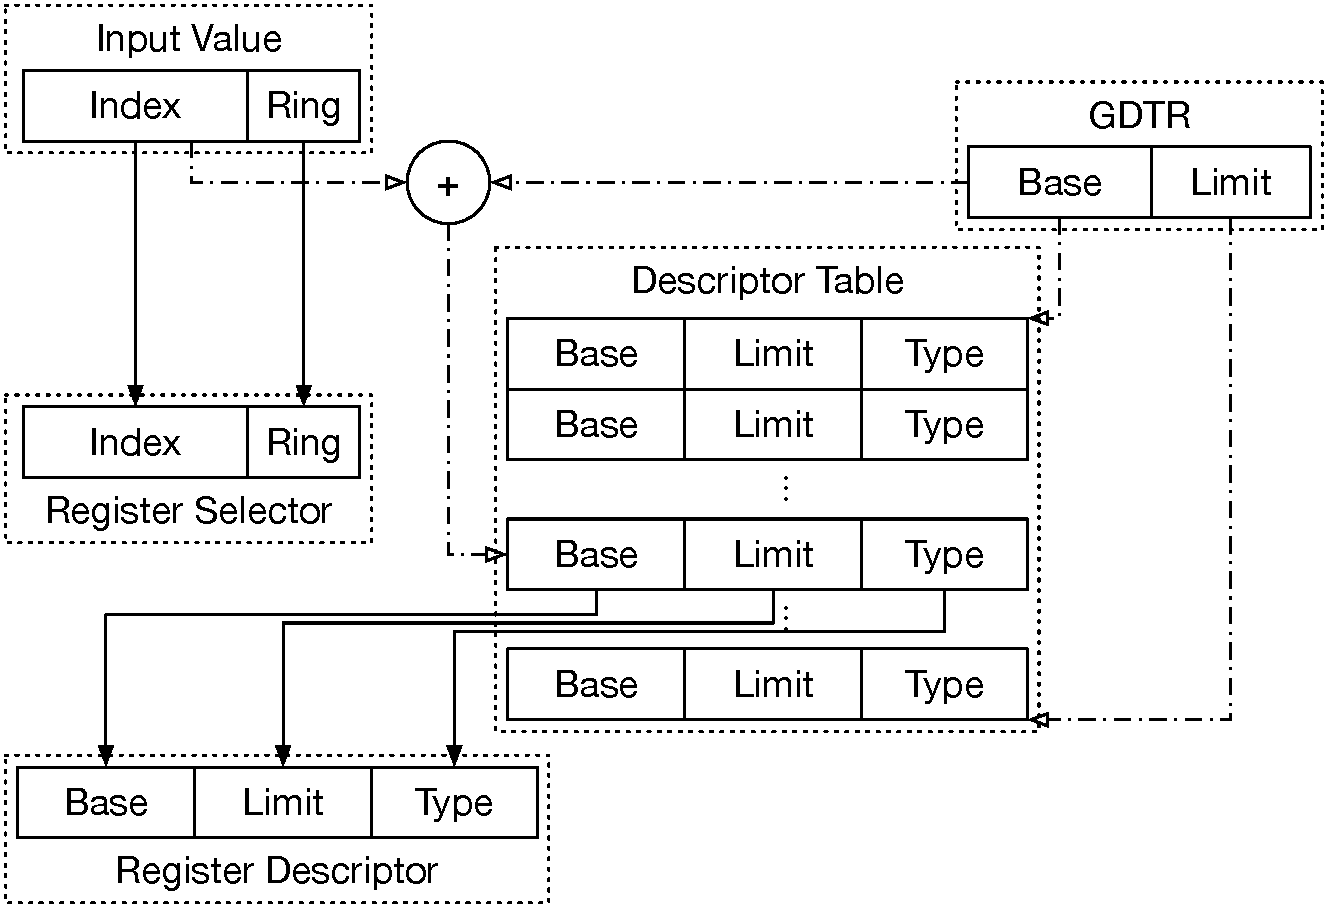
\includegraphics[width=85mm]{figures/cpu_segment.pdf}}
  \caption{
    Loading a segment register. The 16-bit value loaded by software is a
    selector consisting of an index and a ring number. The index selects a GDT
    entry, which is loaded into the descriptor part of the segment register.
  }
  \label{fig:cpu_segment}
\end{figure}

In 64-bit mode, all segment limits are ignored. The base addresses in most
segment registers (CS, DS, ES, SS) are ignored. The base addresses in FS and GS
are used, in order to support thread-local storage.
Figure~\ref{fig:cpu_segmentation} outlines the address computation in this
case. The instruction's address, named \textit{logical address} in the Intel
documentation, is added to the base address in the segment register's
descriptor, yielding the virtual address, also named \textit{linear address}.
The virtual address is then translated (\S~\ref{sec:paging}) to a physical
address.

\begin{figure}[hbt]
  \center{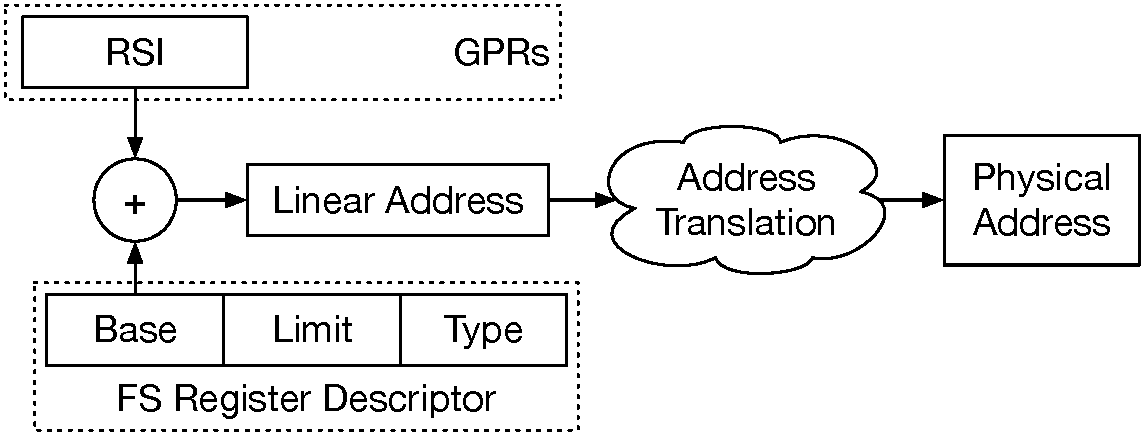
\includegraphics[width=80mm]{figures/cpu_segmentation.pdf}}
  \caption{
    Example address computation process for \texttt{MOV FS:[RDX], 0}.  The
    segment's base address is added to the address in RDX before address
    translation (\S~\ref{sec:paging}) takes place.
  }
  \label{fig:cpu_segmentation}
\end{figure}

Outside the special case of using FS or GS to reference thread-local storage,
the logical and virtual (linear) addresses match, so most of this paper uses
the term ``virtual address'' and ignores segmentation.

Even though CS is not used for segmentation, 64-bit system software needs to
load a valid selector into it. The CPU uses the ring number in the CS selector
to track the current privilege level, and uses one of the type bits to know
whether it's running 64-bit code, or 32-bit code in compatibility mode.

% Null Segment Selector Checking: SDM S 5.4.1, S 5.4.1.1

The DS and ES segment registers are completely ignored, and can have null
selectors loaded in them. The CPU loads a null selector in SS when switching
privilege levels, discussed in \S~\ref{sec:faults}.

% Segment Loading Instructions in IA-32e Mode: SDM S 3.4.4
% Segmentation in IA-32e Mode: SDM S 3.2.4

Modern kernels only use one descriptor table, the \textit{Global Descriptor
Table} (GDT), whose virtual address is stored in the GDTR register. Table~
\ref{fig:gdt_layout} shows a typical GDT layout that can be used by 64-bit
kernels to run both 32-bit and 64-bit applications.

\begin{table}[hbt]
  \center{\begin{tabular}{| l | l |}
  \hline
  \textbf{Descriptor} & \textbf{Selector}\\
  \hline
  Null (must be unused) & 0 \\
  \hline
  Kernel code & 0x08 (index 1, ring 0) \\
  \hline
  Kernel data & 0x10 (index 2, ring 0) \\
  \hline
  User code & 0x1B (index 3, ring 3) \\
  \hline
  User data & 0x1F (index 4, ring 3) \\
  \hline
  TSS & 0x20 (index 5, ring 0) \\
  \hline
  \end{tabular}}
  \caption{
    A typical GDT layout in the 64-bit Intel Architecture.
  }
  \label{fig:gdt_layout}
\end{table}

% TSS Descriptor: SDM S 7.2.2
% TSS Descriptor in 64-bit mode: SDM S 7.2.3
% Task Register: SDM S 7.2.4
% Task Management in 64-bit Mode: SDM S 7.7

The last entry in Table~\ref{fig:gdt_layout} is a descriptor for the
\textit{Task State Segment} (TSS), which was designed to implement hardware
context switching, named \textit{task switching} in the Intel documentation.
The descriptor is stored in the \textit{Task Register} (TR), which behaves like
the other segment registers described above.

Task switching was removed from the 64-bit architecture, but the TR segment
register was preserved, and it points to a repurposed TSS data structure. The
64-bit TSS contains an \textit{I/O map}, which indicates what parts of the I/O
address space can be accessed directly from ring 3, and the
\textit{Interrupt Stack Table} (IST), which is used for privilege level
switching (\S~\ref{sec:faults}).

Modern operating systems do not allow application software any direct access to
the I/O address space, so the kernel sets up a single TSS that is loaded into
TR during early initialization, and used to represent all applications running
under the OS.

\subsection{Privilege Level Switching}
\label{sec:privilege_switches}

Applications software needs a method to invoke the kernel, because it cannot
directly perform privileged operations, such as network or disk I/O. At the
same time, ring 3 software cannot be offered the ability to jump arbitrarily
into kernel code, as that would compromise the kernel's ability to isolate
applications and enforce security invariants.\footnote{For example, when an
application wishes to write a file to the disk, the kernel must check if the
application's user has access to that file. If the ring 3 code could perform
an arbitrary jump in kernel space, it would be able to skip the access check.}
Therefore, the processor has designated methods for switching privilege levels,
which protect the integrity of the privileged software.

This section describes the privilege switching mechanisms that impact the SGX
design, summarized in Figure~\ref{fig:cpu_ring_switch}. Also, understanding the
considerations behind privilege switching is useful when analyzing SGX, because
the process of calling code inside an enclave is similar to switching privilege
levels, as an enclave's code must be able to enforce its own security
invariants, just like an OS kernel.


\subsubsection{System Calls}
\label{sec:syscalls}

% Fast System Calls in 64-Bit Mode: SDM S 5.8.8

\begin{figure}[hbt]
  \center{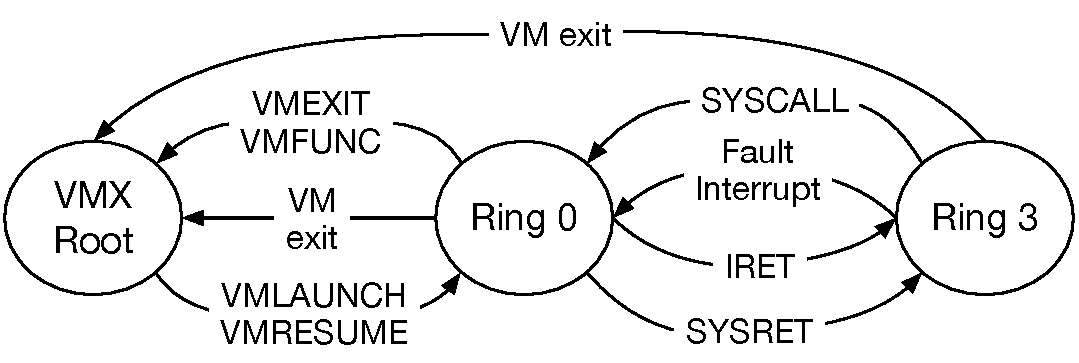
\includegraphics[width=85mm]{figures/cpu_ring_switch.pdf}}
  \caption{
    Modern privilege switching methods in the 64-bit Intel architecture.
  }
  \label{fig:cpu_ring_switch}
\end{figure}

On modern processors, application software uses the SYSCALL instruction to
invoke ring 0 code, and the kernel uses SYSRET to switch the privilege level
back to ring 3. SYSCALL jumps into a predefined kernel location, which is
specified by writing to a pair of architectural MSRs
(\S~\ref{sec:address_spaces}).  MSRs can only be read or written by ring 0
code, so application software cannot modify SYSCALL's MSRs and abuse the
SYSCALL instruction to execute arbitrary kernel code. The SYSRET instruction
switches back to ring 3 and jumps to the address in RCX, which is set by the
SYSCALL instruction. The SYSCALL / SYSRET pair is optimized for speed by
avoiding memory accesses. The design can get away without referencing a stack
because kernel calls are not recursive.


\subsubsection{Faults}
\label{sec:faults}

% Interrupt and Exception Handling: SDM S 6.1, S 6.2
% Access Rights: SDM S 4.6
% Page-Fault Exceptions: SDM S 4.7

The processor also performs a switch from ring 3 to ring 0 when a \textit{
hardware exception} occurs while executing application code. Some exceptions
indicate bugs in the application, whereas other exceptions require kernel
action. A \textit{general protection fault} (\#GP) occurs when software
attempts to perform a disallowed action, such as setting the CR3 register from
ring 3. A \textit{page fault} (\#PF) occurs when address translation encounters
a page table entry whose P flag is 0, or attempting to use a page in a way
inconsistent with the access bits in its page table entry, for example
accessing a page whose S bit is set from ring 3.

% Interrupt Descriptor Table (IDT): SDM S 6.10

When a hardware exception occurs in application code, the CPU performs a ring
switch, and calls the corresponding \textit{exception handler}. For example,
the \#GP handler typically terminates the application's process, while the \#PF
handler reads the swapped out page back into RAM and resumes the application's
execution.

The exception handlers are a part of the OS kernel, and their locations are
specified in the first 32 entries of the Interrupt Descriptor Table (IDT),
whose structure is shown in Table~\ref{fig:idt_entry}. The IDT's physical
address is stored in the IDTR register, which can only be accessed by ring 0
code. Kernels protect the IDT memory using page tables, so that ring 3 software
cannot access it.

\begin{table}[hbt]
  \center{\begin{tabular}{| l | r |}
  \hline
  \textbf{Field} & \textbf{Bits} \\
  \hline
  Handler RIP & 64 \\
  \hline
  Handler CS & 16 \\
  \hline
  Interrupt Stack Table (IST) index & 3 \\
  \hline
  \end{tabular}}
  \caption{
    The essential fields of an IDT entry in 64-bit mode. Each entry points to a
    hardware exception or interrupt handler.
  }
  \label{fig:idt_entry}
\end{table}

Each IDT entry has a 3-bit index pointing into the Interrupt Stack Table (IST),
which is an array of 8 stack pointers stored in the TSS described in
\S~\ref{sec:segments}.

% 64-Bit Mode Stack Frame: SDM S 6.14.2
% IRET in IA-32e Mode: SDM S 6.14.3
% Stack Switching in IA-32e Mode: SDM S 6.14.4
% Interrupt Stack Table: SDM S 6.14.5

When a hardware exception occurs, the execution state may be corrupted, and the
current stack cannot be relied on. Therefore, the CPU first uses the handler's
IDT entry to set up a known good stack. SS is loaded with a null descriptor,
and RSP is set to the IST value pointed by the IDT entry. After switching to a
reliable stack, the CPU pushes the snapshot in Table~\ref{fig:fault_stack} on
the stack, then loads the IDT entry's values into the CS and RIP registers,
which trigger the execution of the exception handler.

\begin{table}[hbt]
  \center{\begin{tabular}{| l | r |}
  \hline
  \textbf{Field} & \textbf{Bits} \\
  \hline
  Exception SS & 64 \\
  \hline
  Exception RSP & 64 \\
  \hline
  RFLAGS & 64 \\
  \hline
  Exception CS & 64 \\
  \hline
  Exception RIP & 64 \\
  \hline
  Exception code & 64 \\
  \hline
  \end{tabular}}
  \caption{
    The snapshot pushed on the handler's stack when a hardware exception
    occurs. IRET restores registers from this snapshot.
  }
  \label{fig:fault_stack}
\end{table}

After the exception handler completes, it uses the \texttt{IRET} (interrupt
return) instruction to load the registers from the on-stack snapshot and switch
back to ring 3.

The Intel architecture gives the fault handler complete control over the parts
of the execution context not listed in Table~\ref{fig:fault_stack}. This
privilege is used by some handlers (e.g., \#GP) to perform context switches
(\S~\ref{sec:registers}) after a process is terminated due to a bug. However,
in the SGX threat model, system software is not trusted, and giving it access
to an enclave's execution context would expose potentially sensitive
information, and present an opportunity to compromise the enclave's integrity.
Therefore, SGX cannot use the current fault handling process, and must modify
it.


\subsubsection{VM Exits}
\label{sec:vm_exits}

If an EPT entry has the P flag set to 0, the CPU performs a VM exit, and the
hypervisor has an opportunity to bring the page into RAM.






\subsection{A Computer Map}

This section maps out a computer using the Intel architecture at three zoom
levels: the motherboard, the CPU, and the execution core, focusing on the
concepts needed to understand SGX and analyze its security properties. Most
details in here are documented in Intel's
\textit{Optimization Reference Manual} \cite{intel2014optimization}.


\subsubsection{The Motherboard}
\label{sec:motherboard}

A computer's components are connected by a printed circuit board called a
\textit{motherboard}, which consists of \textit{sockets} connected by
\textit{buses}. Sockets connect chip-carrying \textit{packages} to the board.
The Intel documentation uses the term ``package'' to specifically refer to a
CPU.

The buses most relevant to SGX (see Figure~\ref{fig:motherboard}) are the
\textit{Quick-Path Interconnect} (QPI) \cite{intel2009qpi}, a network of
point-to-point links that connect processors, the \textit{double data rate}
(DDR) bus that connects a CPU to DRAM, and the \textit{Peripheral Component
Interconnect Express} (PCIe) bus that connects a CPU to peripherals such as a
\textit{Network Interface Card} (NIC).

\begin{figure}[hbt]
  \center{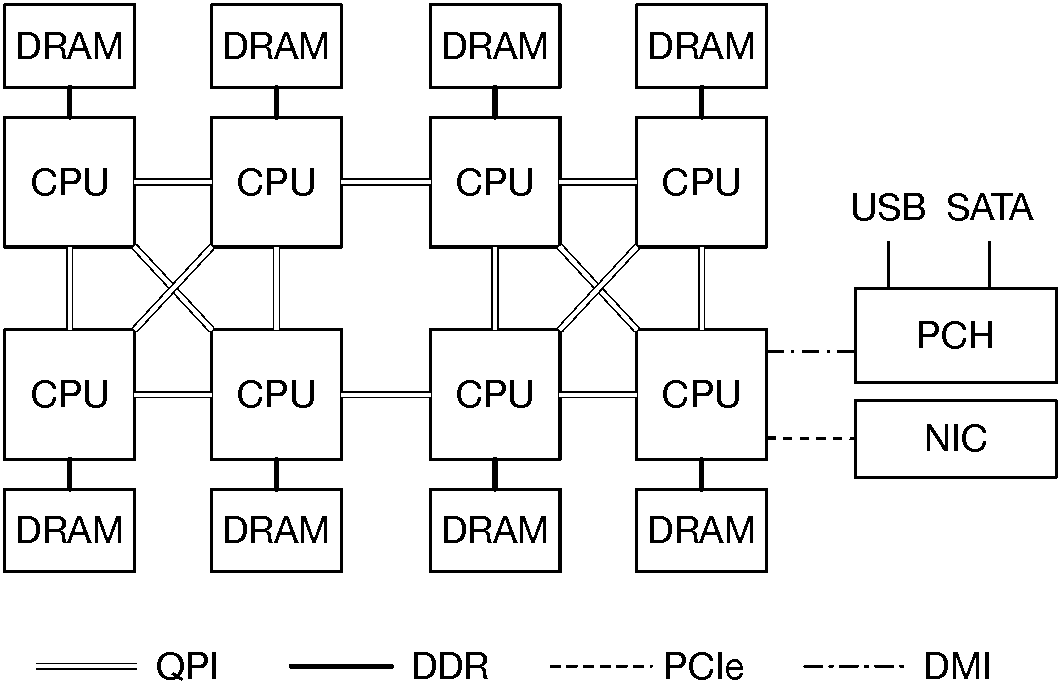
\includegraphics[width=85mm]{figures/motherboard.pdf}}
  \caption{
    The motherboard structures that are most relevant to SGX.
  }
  \label{fig:motherboard}
\end{figure}

The SGX trusted computing base includes the processor package, and excludes the
other hardware in the computer. It follows that SGX must be able to fend off
attacks from rogue devices, such as the PCIe NIC used to compromise Intel TXT
\cite{wojtczuk2011txt}, as well as passive or active bus-tapping attacks, such
as the memory bus tap used to hack the Xbox \cite{huang2003xbox} and the
memory glitching attack that subverted the PlayStation 3 hypervisor
\cite{hotz2010ps3}.


\subsubsection{The Processor}
\label{sec:cpu_die}

An Intel processor's die, illustrated in Figure~\ref{fig:cpu_die}, is divided
into two broad areas: the \textit{core area} implements the instruction
execution pipeline typically associated with CPUs, while the \textit{uncore}
provides functions that were traditionally hosted on separate chips, but are
currently integrated on the CPU die to save power and improve latency.

\begin{figure}[hbt]
  \center{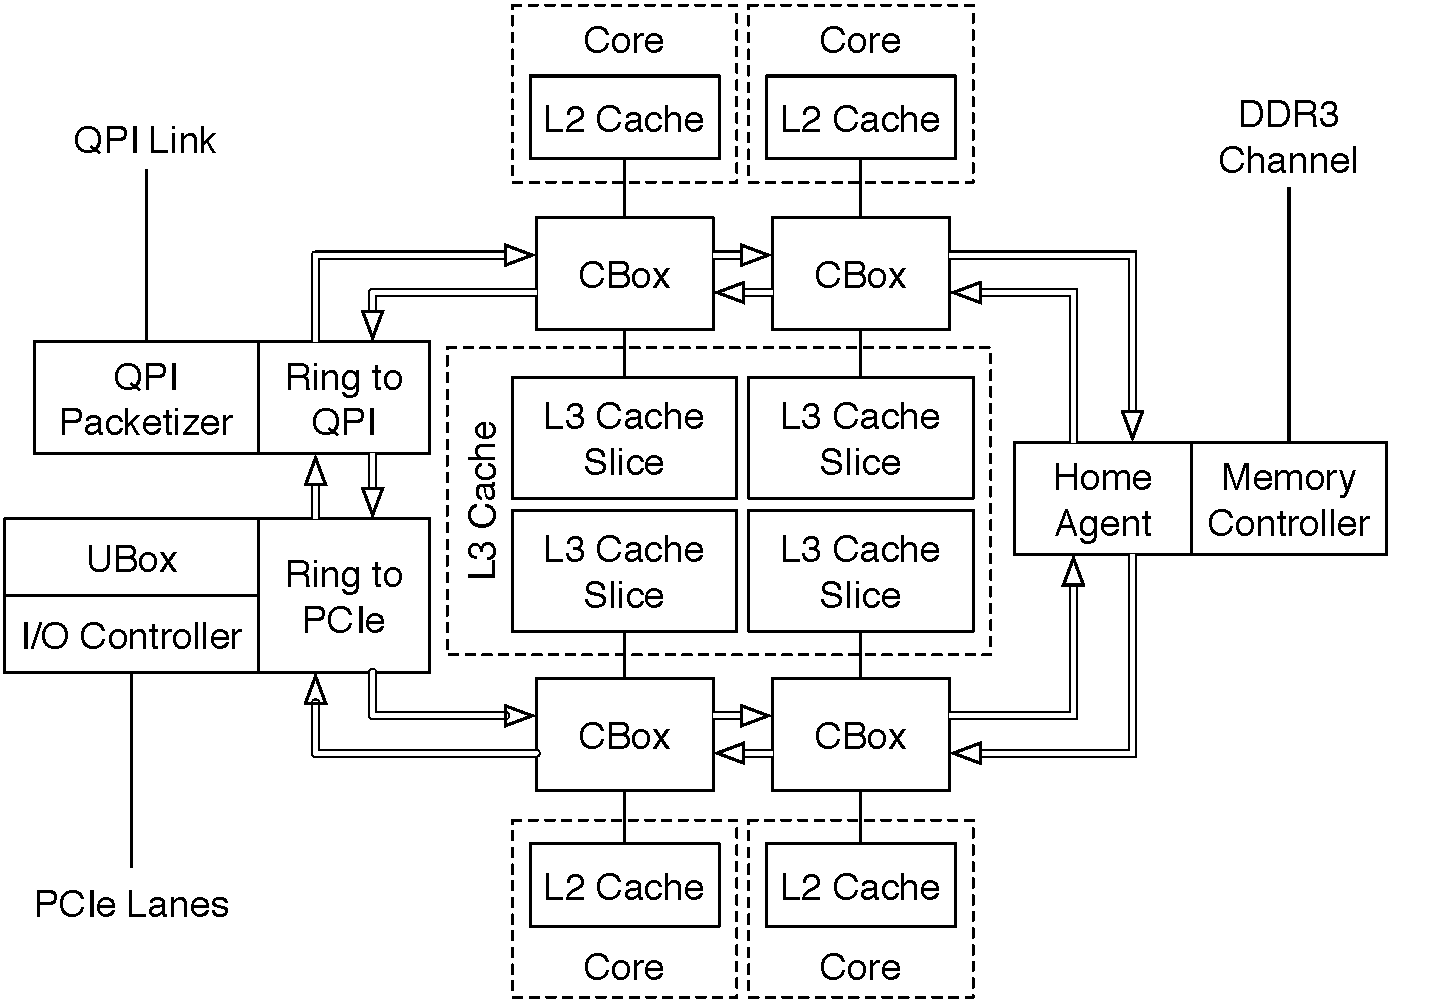
\includegraphics[width=85mm]{figures/cpu_die.pdf}}
  \caption{
    The major components in a modern CPU package. \S~\ref{sec:cpu_die} gives
    an uncore overview. \S~\ref{sec:cpu_core} describes execution cores.
    \S~\ref{sec:cache_coherence} takes a deeper look at the uncore.
  }
  \label{fig:cpu_die}
\end{figure}

% Ring Interconnect and Last Level Cache: Optimization S 2.2.5.3
% System Agent: Optimization S 2.2.6

At a conceptual level, the uncore of modern processors includes a memory
controller that interfaces with the DDR bus, an I/O controller that can
arbitrate the PCIe bus, and a growing number of integrated controllers for
peripherals, such as a NIC and a GPU. The uncore structure is described in some
processor family datasheets \cite{intel2014datasheet, intel2010datasheet}, and
in the overview sections in Intel's uncore performance monitoring documentation
\cite{intel2014uncore, intel2012uncore, intel2010uncore}.

The SGX design relies on the fact that the processor die includes the memory
and I/O controller, and thus can prevent any device from accessing protected
memory areas via \textit{Direct Memory Access} (DMA) transfers.
\S~\ref{sec:cache_coherence} takes a deeper look at the uncore organization and
at the mechanism used by the SGX implementation to protect sensitive memory.


\subsubsection{The Core}
\label{sec:cpu_core}

Virtually all modern Intel processors have core areas consisting of multiple
copies of the execution core circuitry, each of which is called a
\textit{core}.  At the time of this writing, desktop-class Intel CPUs have 4
cores, and server-class CPUs have as many as 18 cores.

Most Intel CPUs feature \textit{hyper-threading}, which means that a core
(shown in Figure~\ref{fig:cpu_core}) has two copies of the register files
backing the execution context described in \S~\ref{sec:registers}, and can
execute two separate streams of instructions simultaneously. Hyper-threading
increases the utilization of the shared fetch, decode and execution units, in
the presence of memory stalls.

\begin{figure}[hbt]
  \center{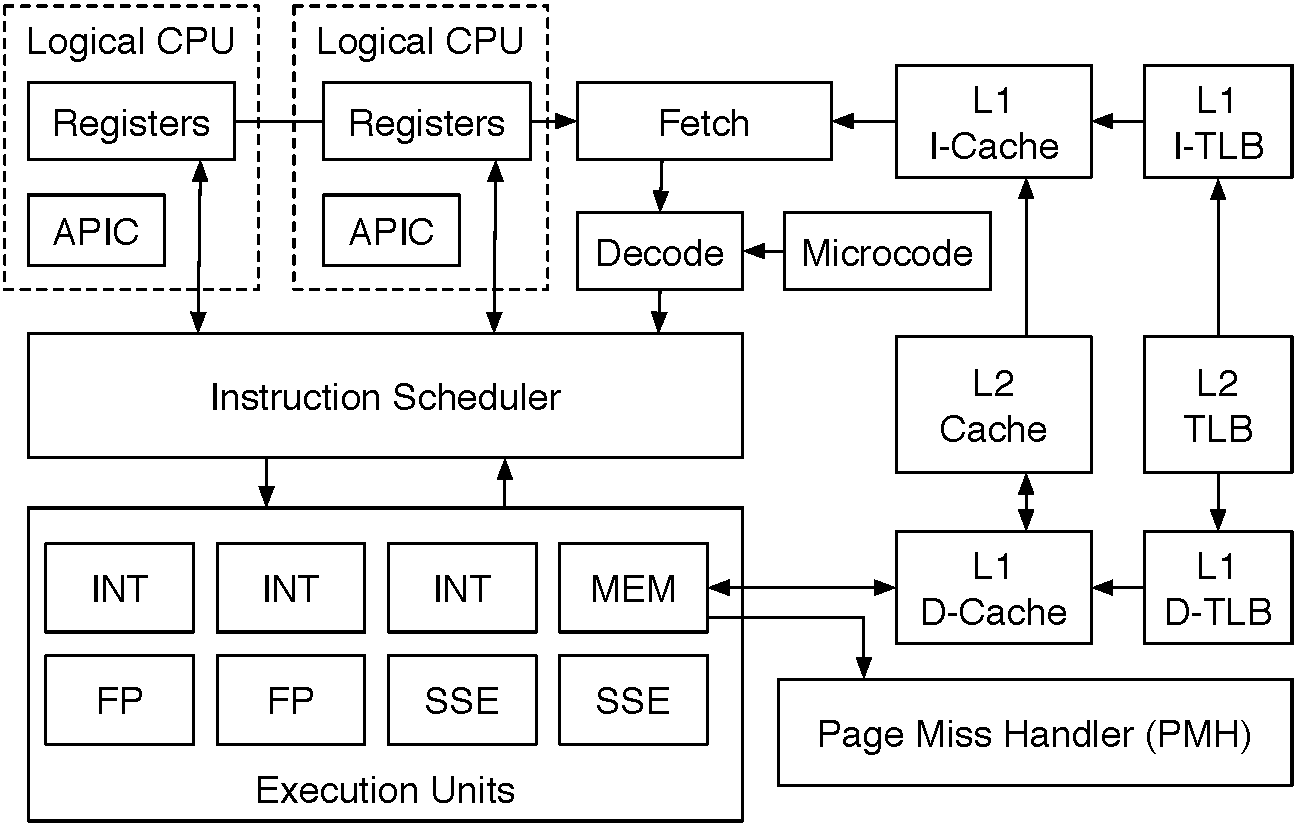
\includegraphics[width=85mm]{figures/cpu_core.pdf}}
  \caption{
    CPU core with two logical processors. Each logical processor has its own
    execution context and local APIC, and they share all the other core
    resources.
  }
  \label{fig:cpu_core}
\end{figure}

A hyper-threaded core is exposed to system software as two \textit{logical
processors}, also named \textit{hardware threads} in the Intel documentation.
The logical processor abstraction allows the code used to distribute work
across processors in a multi-processor system to function without any change on
multi-core hyper-threaded processors.

The high level of resource sharing introduced by hyper-threading introduces a
security vulnerability. Software running on one logical processor can use the
high-performance counter \cite{petters1999making} to get information about the
instructions and memory access patterns of another piece of software that is
executed on the other logical processor in the same core.

\subsection{Out-of-Order and Speculative Execution}
\label{sec:out_of_order}

% Outcome: distinguish observed execution order from program order

CPU cores can execute instructions orders of magnitude faster than DRAM can
read data. Computer architects attempt to bridge this gap by using
hyper-threading (\S~\ref{sec:cpu_die}), out-of-order and speculative execution,
and caching, which is described in \S~\ref{sec:caching}. In CPUs that use
out-of-order execution, the order in which the CPU carries out a program's
instructions (\textit{execution order}) is not necessarily the same as the
order in which the instructions would be executed by a sequential evaluation
system (\textit{program order}).

An analysis of a system's information leakage must take out-of-order execution
into consideration. Any CPU actions observed by an attacker match the execution
order, so the attacker may learn some information by comparing the observed
execution order with a known program order. At the same time, attacks that try
to infer a victim's program order based on actions taken by the CPU must
account for out-of-order execution as a source of noise.

This section summarizes the out-of-order and speculative execution concepts
used when reasoning about a system's security properties.
\cite{patterson2013architecture} and \cite{hennessy2012architecture} cover the
concepts in great depth, while Intel's optimization manual
\cite{intel2014optimization} provides details specific to Intel CPUs.

% The Haswell Microarchitecture: Optimization S 2.1

Figure~\ref{fig:cpu_out_of_order} provides a more detailed view of the CPU core
components involved in out-of-order execution, and omits some less relevant
details from Figure~\ref{fig:cpu_core}.

\begin{figure}[hbt]
  \centering
  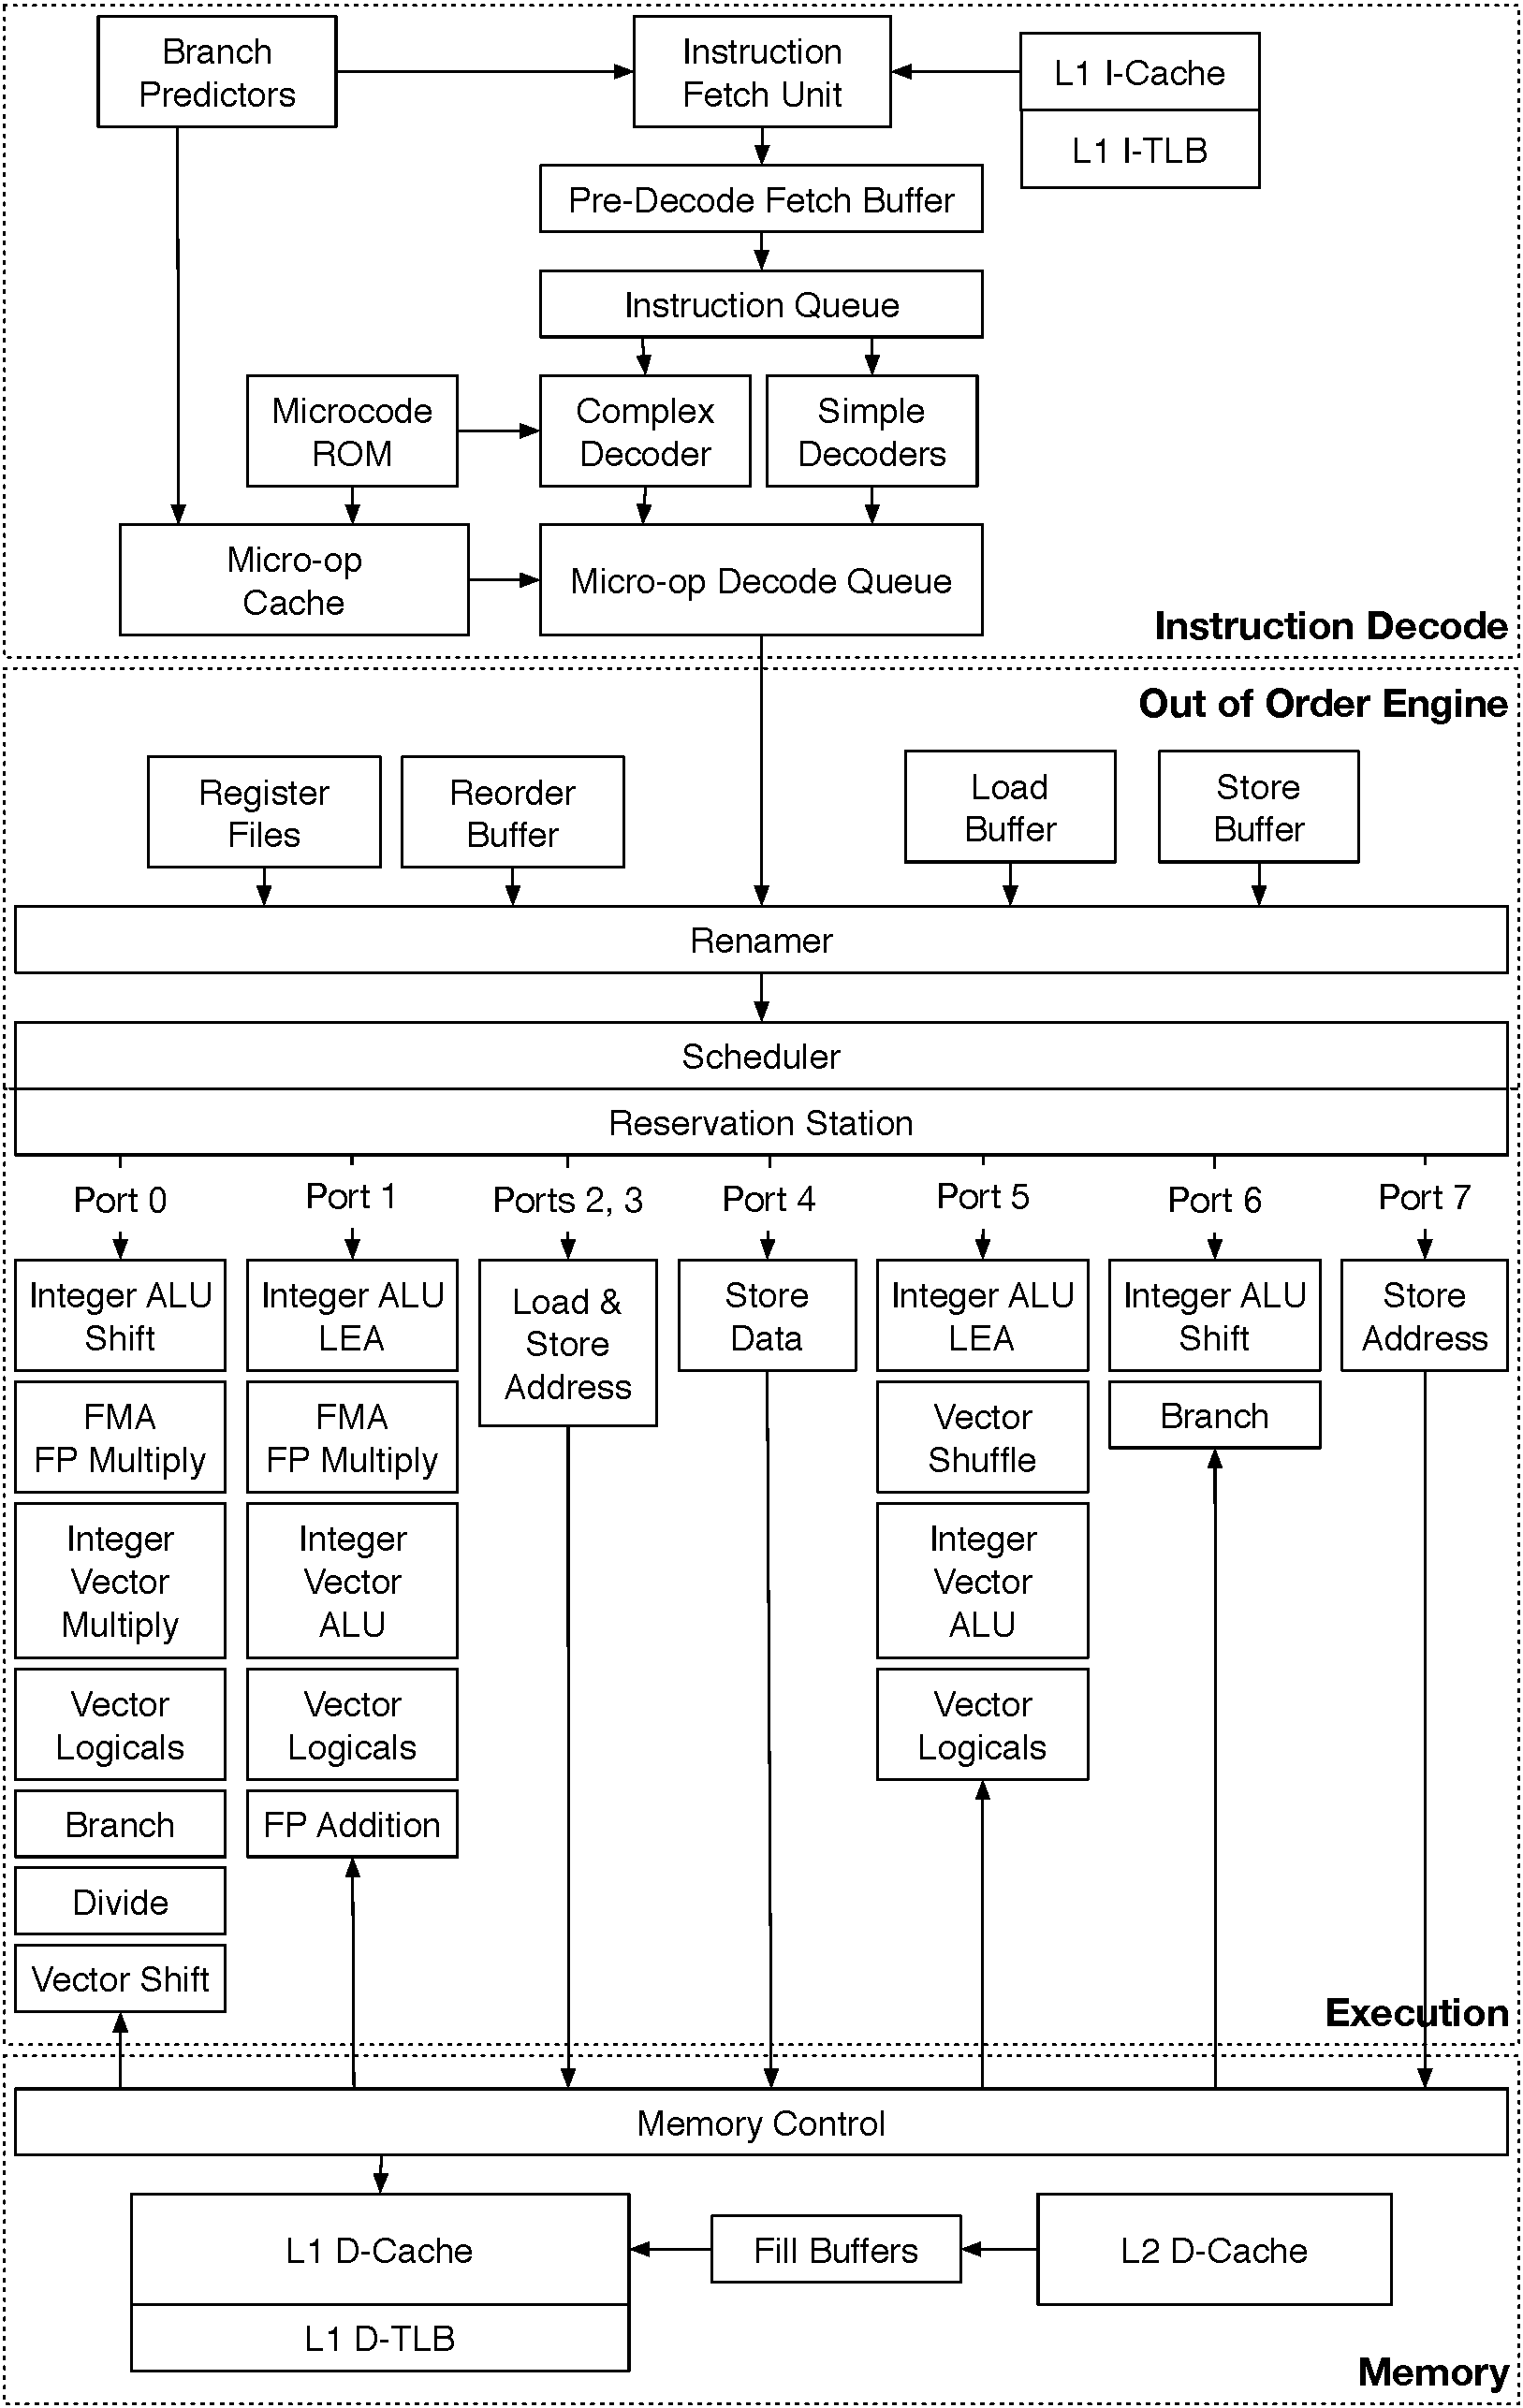
\includegraphics[width=87mm]{figures/cpu_out_of_order.pdf}
  \caption{
    The structures in a CPU core that are relevant to out-of-order and
    speculative execution. Instructions are decoded into micro-ops, which are
    scheduled on one of the execution unit's ports. The branch predictor
    enables speculative execution when a branch is encountered.
  }
  \label{fig:cpu_out_of_order}
\end{figure}

% Intel Microarchitecture Code Name Sandy Bridge Pipeline Overview:
%     Optimization S 2.2.1
% The Front End: Optimization S 2.2.2

The Intel architecture defines a \textit{complex instruction set} (CISC).
However, virtually all modern CPUs are architected following \textit{reduced
instruction set} (RISC) principles. This is accomplished by having the
instruction decode stages break down each instruction into \textit{micro-ops},
which resemble RISC instructions. The other stages of the execution pipeline
work exclusively with micro-ops.


\subsubsection{Out-of-Order Execution}

% Out of Order Engine: Optimization S 2.2.23
% The Execution Core: S 2.2.4

Different types of instructions require different logic circuits, called
\textit{functional units}. For example, the arithmetic logic unit (ALU), which
performs arithmetic operations, is completely different from the load store
unit, which peforms memory operations. Different circuits can be used at the
same time, so each CPU core can execute multiple micro-ops in parallel.

The core's out-of-order engine receives decoded micro-ops, identifies the
micro-ops that can execute in parallel, assigns them to functional units, and
combines the outputs of the units so that the results are equivalent to having
the micro-ops executed sequentially in the order in which they come from the
decode stages.

For example, consider the sequence of pseudo micro-ops\footnote{The set of
micro-ops used by Intel CPUs is not publicly documented. The fictional examples
in this section suffice for illustration purposes.} in
Table~\ref{fig:out_of_order_micro_ops} below. The \texttt{OR} uses the result
of the \texttt{LOAD}, but the \texttt{ADD} does not. Therefore, a good
scheduler can have the load store unit execute the \texttt{LOAD} and the ALU
execute the \texttt{ADD}, all in the same clock cycle.

\begin{table}[hbt]
  \centering
  \begin{tabular}{| l | l | l |}
  \hline
  \textbf{\#} & \textbf{Micro-op} & \textbf{Meaning}\\
  \hline
  1 & \texttt{LOAD RAX, RSI} & RAX $\leftarrow$ DRAM[RSI]\\
  \hline
  2 & \texttt{OR RDI, RDI, RAX} & RDI $\leftarrow$ RDI $\lor$ RAX\\
  \hline
  3 & \texttt{ADD RSI, RSI, RCX} & RSI $\leftarrow$ RSI + RCX\\
  \hline
  4 & \texttt{SUB RBX, RSI, RDX} & RBX $\leftarrow$ RSI - RDX\\
  \hline
  \end{tabular}
  \caption{
    Pseudo micro-ops for the out-of-order execution example.
  }
  \label{fig:out_of_order_micro_ops}
\end{table}

% Renamer: Optimization S 2.2.3.1

The out-of-order engine in recent Intel CPUs works roughly as follows.
Micro-ops received from the decode queue are written into a \textit{reorder
buffer} (ROB) while they are \textit{in-flight} in the execution unit. The
\textit{register allocation table} (RAT) matches each register with the last
reorder buffer entry that updates it. The \textit{renamer} uses the RAT to
rewrite the source and destination fields of micro-ops when they are written in
the ROB, as illustrated in Tables \ref{fig:out_of_order_rob} and
\ref{fig:out_of_order_rat}. Note that the ROB representation makes it easy to
determine the dependencies between micro-ops.

\begin{table}[hbt]
  \centering
  \begin{tabular}{| l | l | l | l | l |}
  \hline
  \textbf{\#} & \textbf{Op} & \textbf{Source 1} & \textbf{Source 2} &
  \textbf{Destination}\\
  \hline
  1 & LOAD & RSI & $\emptyset$ & RAX \\
  \hline
  2 & OR & RDI & ROB \#1 & RSI \\
  \hline
  3 & ADD & RSI & RCX & RSI \\
  \hline
  4 & SUB & ROB \# 3 & RDX & RBX \\
  \hline
  \end{tabular}
  \caption{
    Data written by the renamer into the reorder buffer (ROB), for the
    micro-ops in Table~\ref{fig:out_of_order_micro_ops}.
  }
  \label{fig:out_of_order_rob}
\end{table}

\begin{table}[hbt]
  \centering
  \begin{tabular}{| l | r | r | r | r | r | r |}
  \hline
  \textbf{Register} & RAX & RBX & RCX & RDX & RSI & RDI \\
  \hline
  \textbf{ROB \#} & \#1 & \#4 & $\emptyset$ & $\emptyset$ & \#3 & \#2 \\
  \hline
  \end{tabular}
  \caption{
    Relevant entries of the register allocation table after the micro-ops in
    Table~\ref{fig:out_of_order_micro_ops} are inserted into the ROB.
  }
  \label{fig:out_of_order_rat}
\end{table}

% Scheduler: Optimization S 2.2.3.2

The scheduler decides which micro-ops in the ROB get executed, and places them
in the \textit{reservation station}. The reservation station has one port
for each functional unit that can execute micro-ops independently. Each
reservation station port port holds one micro-op from the ROB. The reservation
station port waits until the micro-op's dependencies are satisfied and forwards
the micro-op to the functional unit. When the functional unit completes
executing the micro-op, its result is \textit{written back} to the ROB, and
forwarded to any other reservation station port that depends on it.

The ROB stores the results of completed micro-ops until they are
\textit{retired}, meaning that the results are \textit{committed} to the
register file and the micro-ops are removed from the ROB. Although micro-ops
can be executed out-of-order, they must be retired in program order, in order
to handle exceptions correctly. When a micro-op causes a hardware exception
(\S~\ref{sec:faults}), all the following micro-ops in the ROB are
\textit{squashed}, and their results are discarded.

In the example above, the \texttt{ADD} can complete before the \texttt{LOAD},
because it does not require a memory access. However, the \textit{ADD}'s result
cannot be committed before \texttt{LOAD} completes. Otherwise, if the
\textit{ADD} is committed and the \textit{LOAD} causes a page fault, software
will observe an incorrect value for the  RSI register.

% Load and Store Operation Overview: Optimization S 2.2.5

The ROB is tailored for discovering register dependencies between micro-ops.
However, micro-ops that execute out-of-order can also have memory dependencies.
For this reason, out-of-order engines have a \textit{load buffer} and a
\textit{store buffer} that keep track of in-flight memory operations and are
used to resolve memory dependencies.


\subsubsection{Speculative Execution}

% Branch Prediction: Optimization S 2.2.2.3

Branch instructions, also called \textit{branches}, change the instruction
pointer (RIP, \S~\ref{sec:registers}), if a condition is met (\textit{the
branch is taken}). They implement conditional statements (\texttt{if}) and
looping statements, such as \texttt{while} and \texttt{for}. The most
well-known branching instructions in the Intel architecture are in the
\texttt{j\textit{cc}} family, such as \texttt{je} (jump if equal).

Branches pose a challenge to the decode stage, because the instruction that
should be fetched after a branch is not known until the branching condition is
evaluated. In order to avoid stalling the decode stage, modern CPU designs
include \textit{branch predictors} that use historical information to guess
whether a branch will be taken or not.

When the decode stage encounters a branch instruction, it asks the branch
predictor for a guess as to whether the branch will be taken or not. The
decode stage bundles the branch condition and the predictor's guess into a
branch check micro-op, and then continues decoding on the path indicated by the
predictor. The micro-ops following the branch check are marked as
\textit{speculative}.

When the branch check micro-op is executed, the branch unit checks whether the
branch predictor's guess was correct. If that is the case, the branch check is
retired successfully. The scheduler handles \textit{mispredictions} by
squashing all the micro-ops following the branch check, and by signaling the
instruction decoder to flush the micro-op decode queue and start fetching the
instructions that follow the correct branch.

% Data Prefetching: Optimization S 2.2.5.4

Modern CPUs also attempt to predict memory read patterns, so they can
\textit{prefetch} the memory locations that are about to be read into the
cache. Prefetching minimizes the latency of successfully predicted read
operations, as their data will already be cached. This is accomplished by
exposing circuits called prefetchers to memory accesses and cache misses. Each
prefetcher can recognize a particular access pattern, such as squentially
reading an array's elements. When memory accesses match the pattern that a
prefetcher was built to recognize, the prefetcher loads the cache line
corresponding to the next memory access in its pattern.

\subsection{Cache Memories}
\label{sec:caching}

At the time of this writing, CPU cores can process data $\approx 200\times$
faster than DRAM can supply it. This gap is bridged by an hierarchy of cache
memories, which are orders of magnitude smaller and an order of magnitude
faster than DRAM. This section reviews the key concepts needed to understand
\textit{cache timing attacks} \cite{banescu2011cache}, which can be used to
learn about an application's memory access patterns. \cite{smith1982cache},
\cite{patterson2013architecture} and \cite{hennessy2012architecture} all
provide good backgrounds on low-level cache implementation concepts.

At a high level, caches exploit the high locality in the memory access patterns
of most applications to hide the main memory's (relatively) high latency. By
\textit{caching} (storing a copy of) the most recently accessed code and data,
caches can be used to satisfy 90\%-99\% of an application's memory accesses.

In an Intel processor, the \textit{first-level} (L1) cache consists of a
separate data cache (D-cache) and an instruction cache (I-cache). The
instruction fetch and decode stage is directly connected to the L1 I-cache, and
uses it to read the streams of instructions for the core's logical processors.
Micro-ops that read from or write to memory are executed by the memory unit
(MEM in Figure~\ref{fig:cpu_core}), which is connected to the L1 D-cache and
forwards memory accesses to it.

Figure \ref{fig:cache_lookup} illustrates the steps taken by a cache when it
receives a memory access. First, a \textit{cache lookup} uses the memory
address to determine if the corresponding data exists in the cache. A
\textit{cache hit} occurs when the address is found, and the cache can resolve
the memory access quickly. Conversely, if the address is not found, a
\textit{cache miss} occurs, and a \textit{cache fill} is required to resolve
the memory access. When doing a fill, the cache forwards the memory access to
the next level of the memory hierarchy and caches the response. Under most
circumstances, a cache fill also triggers a \textit{cache eviction}, in which
some data is removed from the cache to make room for the data coming from the
fill. If the data that is evicted has been modified since it was loaded in the
cache, it must be \textit{written back} to the next level of the memory
hierarchy.

\begin{figure}[hbt]
  \centering
  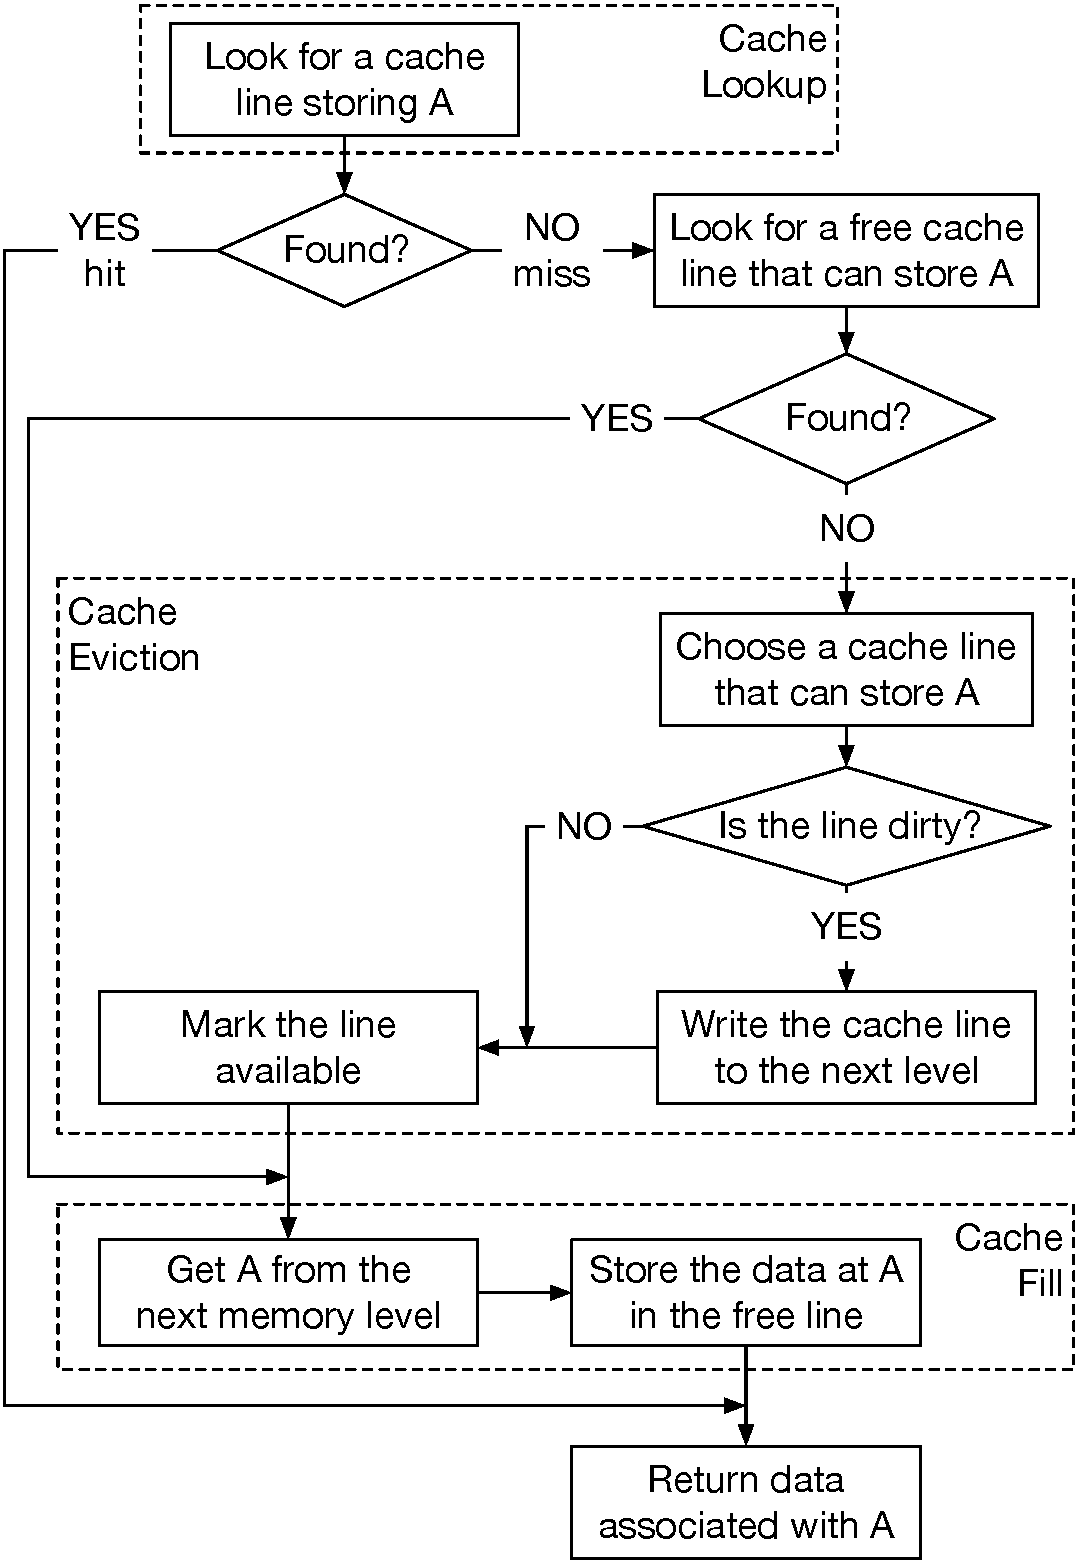
\includegraphics[width=80mm]{figures/cache_lookup.pdf}
  \caption{
    The steps taken by a cache memory to resolve an access to a memory address
    A. A normal memory access (to cacheable DRAM) always triggers a cache
    lookup. If the access misses the cache, a fill is required, and a
    write-back might be required.
  }
  \label{fig:cache_lookup}
\end{figure}

Unfortunately, caches create a dependency between the location of a memory
access and the time it takes to perform the access. A cache miss requires
at least one memory access to the next level cache, and might require a second
memory access if a write-back occurs. The related work presented in
\cite{banescu2011cache} shows that it is practical to use the timing
differences between hits and misses to learn the memory access patterns of a
target thread, as long as an attacker thread shares a cache with the target
thread. The target's memory access patterns, in turn, can reveal private
information, such as whether certain bits in an encryption key are set or not.

Table~\ref{fig:cache_timings} shows the key characteristics of the memory
hierarchy implemented by modern Intel CPUs. Each core has its own L1 and L2
cache (see Figure~\ref{fig:cpu_core}), while the L3 cache is in the CPU's
uncore (see Figure~\ref{fig:cpu_die}), and is shared by all the cores in the
package.

% Cache and Memory Subsystem: Optimization S 2.1.4
% Cache Hierarchy: Optimization S 2.2.5

\begin{table}[hbt]
  \centering
  \begin{tabular}{| l | r | r |}
  \hline
  \textbf{Memory} & \textbf{Size} & \textbf{Access Time}\\
  \hline
  Core Registers & 1~KB & no latency \\
  \hline
  L1 D-Cache & 32~KB & 4 cycles \\
  \hline
  L2 Cache & 256~KB & 10 cycles \\
  \hline
  L3 Cache & 8~MB & 40-75 cycles \\
  \hline
  DRAM & 16~GB & 60 ns \\
  \hline
  \end{tabular}
  \caption{
    Approximate sizes and access times for each level in the memory
    hierarchy of an Intel processor, from \cite{intel2010perfanalysis}. Memory
    sizes and access times differ by orders of magnitude across the different
    levels of the hierarchy. This table does not cover multi-processor systems.
  }
  \label{fig:cache_timings}
\end{table}

A cache timing attack that aims at the L2 cache would have to rely on the
system software to schedule a software thread on a logical processor in the
same core as the target software, whereas an attack on the L3 cache can be
performed using any logical processor on the same CPU. This implies that L3
cache attacks are feasible in an IaaS environment, whereas L2 cache attacks
become a possibility when running sensitive software on a user's desktop.

Our analysis of SGX concludes that it is vulnerable to cache timing attacks,
which can be used to obtain high-resolution memory access patterns for the
software running inside an SGX enclave.

\subsection{Interrupts}
\label{sec:interrupts}

Peripherals use \textit{interrupts} to signal the occurrence of an event that
must be handled by system software. For example, a keyboard issues interrupts
when a key is pressed or depressed. System software also relies on interrupts
to implement preemptive multi-threading. This section presents the details
needed to understand the concerns and tools that interrupts bring to the SGX
implementation.

% Advanced Programmable Interrupt Controller (APIC): SDM S 10
% Message Signalled Interrupts (MSI): SDM S 10.11

Peripherals use bus-specific protocols to signal interrupts. For example, PCIe
relies on \textit{Message Signaled Interrupts} (MSI), which are memory writes
issued to specially designed memory addresses. The bus-specific interrupt
signals are received by the \textit{I/O Advanced Programmable Interrupt
Controller} (IOAPIC) in the PCH, shown in Figure~\ref{fig:motherboard}.

% Local APIC ID: SDM S 10.4.6
% Extended xAPIC (x2APIC): SDM S 10.12

The IOAPIC routes interrupt signals to one or more \textit{Local Advanced
Programmable Interrupt Controllers} (LAPICs). As shown in
Figure~\ref{fig:cpu_die}, each logical CPU has a LAPIC that can receive
interrupt signals from the IOAPIC. The IOAPIC routing process assigns each
interrupt to an 8-bit \textit{interrupt vector}, used to identify the interrupt
sources, and a 32-bit \textit{APIC ID} used to identify the LAPIC that receives
the interrupt.

% Handling Interrupts: SDM S 10.8

Each LAPIC uses a 256-bit \textit{Interrupt Request Register} (IRR) to track
the un-serviced interrupts that it has received, based on the interrupt vector
number. When the corresponding logical processor is available, the LAPIC copies
the highest-priority un-serviced interrupt vector to the
\textit{In-Service Register} (ISR), and invokes the logical processor's
interrupt handling process.

% Issuing Interprocessor Interrupts: SDM S 10.6
% Interrupt Command Register (ICR): SDM S 10.6.1

At the architectural level, interrupt handling reuses many of the mechanisms in
fault handling (\S~\ref{sec:faults}). The interrupt vector number in the
LAPIC's ISR is used to locate an interrupt handler in the IDT, and the handler
is invoked, possibly after a privilege switch is performed. The interrupt
handler does the processing that the device requires, and then writes the
LAPIC's \textit{End Of Interrupt} (EOI) register to signal the fact that it has
completed handling the interrupt.

Interrupts are treated like faults, so interrupt handlers have full control
over the execution environment of the application being interrupted. This is
used to implement pre-emptive multi-threading, which relies on a clock device
that generates interrupts periodically, and on an interrupt handler that
performs context switches. While useful for multi-threading, this aspect of the
architecture also implies SGX design must include changes to the interrupt
handling process, in order to protect an enclave's execution state from an
interrupt handler that is invoked while an enclave's code is executing.

System software can cause an interrupt on any logical processor by writing the
target processor's APIC ID into the \textit{Interrupt Command Register} (ICR)
of the LAPIC associated with the logical processor that the software is runing
on. These interrupts, called \textit{Inter-Processor Interrupts} (IPI), are
needed to implement TLB shoot-downs (\S~\ref{sec:tlbs}). The IPI mechanism can
also be used to send SMI interrupts, which opens up an avenue for a malicious
kernel or hypervisor to mount a SMM mode (\S~\ref{sec:rings}) attack.

\subsection{The Boot Process}
\label{sec:booting}

When a computer is powered up, it undergoes a \textit{bootstrapping} process,
also called \textit{booting}, for simplicity. Although many steps in the boot
process depend on the motherboard and components in a computer, the process
does follow a high-level structure that is prescribed in the SDM. This section
provides the details needed to analyze SGX's security properties.
\cite{intel2010booting} provides a good reference on the entire booting
process.

% Initialization Overview: SDM S 9.1

Right after a computer is powered up, all the logical processors (LPs) on the
motherboard undergo \textit{hardware initialization}, which invalidates the
caches (\S~\ref{sec:caching}) and TLBs (\S~\ref{sec:tlbs}), performs a
\textit{Built-In Self Test} (BIST), and sets all the registers
(\S~\ref{sec:registers}) to pre-specified values.

% Multiple-Processor Initialization: SDM S 8.4
% BSP and AP Processors: SDM S 8.4.1
% MP Initialization Protocol Algorithms for MP Systems: SDM S 8.4.3
% An ivy bridge CPUID: family 06h, extended model 3, model 58, stepping 9

After hardware initialization, the LPs perform the Multi-Processor (MP)
initialization algorithm, which results in one LP being selected as the
\textit{bootstrap processor} (BSP), and all the other LPs being classified as
\textit{application processors} (APs).

According to the SDM, the details of the MP initialization algorithm for recent
CPUs depend on the motherboard and firmware. In principle, after completing
hardware initialization, all LPs attempt to issue a special no-op transaction
on the QPI bus. A single LP will suceed in issuing the no-op, thanks to
the QPI arbitration mechanism, and to the UBox (\S~\ref{sec:cache_coherence})
in each CPU package, which also serves as a ring arbiter. The arbitration
priority of each LP is based on its APIC ID APIC ID (\S~\ref{sec:interrupts}),
which is provided by the motherboard when the system powers up. The LP that
issues the no-op becomes the BSP. Upon failing to issue the no-op, the other
LPs become APs, and enter the \textit{wait-for-SIPI} state.

% Typical BSP Initialization Sequence: SDM S 8.4.4.1

The BSP sets its RIP register to point to the firmware reset code, which must
be present at 0xFFFFFFF0 (16 bytes below the 4 GB mark). This is accomplished
by having the initial SAD (\S~\ref{sec:cache_coherence}) and PCH
(\S~\ref{sec:motherboard}) configurations map the 4 KB below the 4 GB mark of
the memory address space (\S~\ref{sec:address_spaces}) to the SPI flash chip
that stores the motherboard's firmware.

\cite{intel2010booting} and \cite{coreboot2015manual} describe the
initialization steps performed by the firmware, from an implementor's
perspective. A few steps are interesting from the perspective of SGX and
caching attacks.

% Preventing Caching: SDM S 11.5.3

When the BSP starts executing firmware code, DRAM is not available. The
firmware places the BSP in \textit{Cache-as-RAM} (CAR) mode to be able to use a
call stack and other high-level constructs. Ater CAR is enabled, the memory
initialization code, which is typically Intel's \textit{Memory Reference Code}
(MRC), is loaded into the cache. When executed, the memory initialization code
discovers the DRAM chips connected to the motherboard and sets them up, and
enables and configures the memory controllers.

% Typical AP Initialization Sequence: SDM S 8.4.4.2


\subsection{CPU Microcode}
\label{sec:microcode}

% Outcome: evaluating the cost of architectural modifications

The Intel architecture features a large instruction set. Some instructions are
used infrequently, and some instructions are very complex, which makes it
impractical for an execution core to handle all the instructions in hardware.
Intel CPUs use a \textit{microcode} table to break down rare and complex
instructions into sequences of simpler instructions. Architectural extensions
that only require microcode changes are siginificantly cheaper to implement
and validate than extensions that require changes in the CPU's circuitry.

It follows that a good understanding of what can be done in microcode is
crucial to evaluating the cost of security features that rely on architecture
extensions. Furthermore, the limitations of microcode are sometimes the
reasoning behind seemingly arbitrary architecture design decisions.

The first sub-section below presents the relevant facts pertaining to microcode
in Intel's optimization reference \cite{intel2014optimization} and SDM. The
following subsections summarize information gleaned from Intel's patents and
other researchers' findings.


\subsubsection{The Role of Microcode}
\label{sec:microcode_role}

% Legacy Decode Pipeline (Instruction Decode): Optimization S 2.2.2.1
% Instruction Decode: Optimization S 2.3.2.4
% Front End Overview: Optimization S 2.4.2
% Understanding the Sources of the Micro-Op Queue: SDM S B.3.7.2

The frequently used instructions in the Intel architecture are handled by the
core's fast path, which consists of simple decoders (\S~\ref{sec:out_of_order})
that can emit at most 4 micro-ops per instruction. Infrequently used
instructions and instructions that require more than 4 micro-ops use a slower
decoding path that relies on a sequencer to read micro-ops from a
\textit{microcode store ROM} (MSROM).

The 4 micro-ops limitation can be used to guess intelligently whether an
architectural feature is implemented in microcode. For example, it is safe to
assume that \texttt{XSAVE} (\S~\ref{sec:registers}), which was takes over 200
micro-ops on recent CPUs \cite{fog2014microops}, is most likely performed in
microcode, whereas simple arithmetic and memory accesses are handled directly
by hardware.

% Assists: Optimization S B.3.5.2

The core's execution units handle common cases in fast paths implemented in
hardware. When an input cannot be handled by the fast paths, the execution
unit issues a \textit{microcode assist}, which points the microcode sequencer
to a routine in microcode that handles the edge cases. The most common cited
example in Intel's documentation is floating point instructions, which issue
assists to handle denormalized inputs.

The \texttt{REP MOVS} family of instructions, also known as \textit{string
instructions} because of their use in \texttt{strcpy}-like functions, operate
on variable-sized arrays. These instructions can handle small arrays in
hardware, and issue microcode assists for larger arrays.

% Microcode Update Facilities: SDM S 9.11
% Responsibilities of the BIOS: SDM 9.11.8.1

Modern Intel processors implement a microcode update facility. The SDM
describes microcode updates from the perspective of an OS kernel and
hypervisor. Each core can be updated independently, and the updates must be
reapplied on each boot cycle. A core can be updated multiple times, but each
update must have a bigger version than the core's current version. The latest
SDM at the time of this writing states that a microcode update is up to 16 KB
in size.

Processor engineers prefer to build new architectural features as microcode
extensions, because microcode can be iterated on much faster than hardware,
which reduces development cost \cite{intel2008genetic, intel2012clusters}. The
update facility further increases the appeal of microcode, as some classes of
bugs can be fixed after a CPU has been released.

Intel patents \cite{intel2013patent1, intel2013patent2} describing Software
Guard Extensions (SGX) disclose that SGX is entirely implemented in microcode,
except for the memory encryption engine. A description of SGX's implementation
could provide great insights into Intel's microcode, but, unfortunately, the
SDM chapters covering SGX do not include such a description. We therefore rely
on other public information sources about the role of microcode in the
security-sensitive areas covered by previous sections, namely memory
management~(\S~\ref{sec:paging}, \S~\ref{sec:tlbs}), the handling of hardware
exceptions~(\S~\ref{sec:faults}) and interrupts~(\S~\ref{sec:interrupts}), and
platform initialization~(\S~\ref{sec:booting}).

% Precise Event Based Sampling (PEBS): SDM S 18.7.1.1
% At-Retirement Counting: SDM S 18.13.6
% Performance Monitoring Events for the 4th Generation Intel Core Processors:
%     SDM S 19.3

The use of microcode assists can be measured using the
\textit{Precise Event Based Sampling} (PEBS) feature in recent Intel
processors. PEBS provides counters for the number of micro-ops coming from
MSROM, including complex instructions and assists, counters for the numbers of
assists associated with some micro-op classes (SSE and AVX stores and
transitions), and a counter for assists generated by all other micro-ops.

The PEBS feature itself is implemented using microcode assists (this is implied
in the SDM and confirmed by \cite{intel2014pebs}) when it needs to write the
execution context into a PEBS record. Given the wide range of features
monitored by PEBS counters, we assume that all execution units in the core can
issue microcode assists, which are performed at micro-op retirement (confirmed
by \cite{intel1997events}).

% Conditional SIMD Packed Loads and Stores: Optimization S 11.9

Intel's optimization manual describes one more interesting assist, from a
memory system perspective. SIMD masked loads (using \texttt{VMASKMOV}) read a
series of data elements from memory into a vector register. A mask register
decides whether elements are moved or ignored. If the memory address overlaps
an invalid page (e.g., the P flag is 0, \S~\ref{sec:paging}), a microcode
assist is issued, even if the mask indicates that no element from the invalid
page should be read. The microcode checks whether the elements in the invalid
page have the corresponding mask bits set, and either performs the load or
issues a page fault.

% IA32_MCG Extended Machine Check State MSRs: SDM S 15.3.2.6

The description of machine checks in the SDM mentions page assists and page
faults in the same context. We assume that the page assists are issued in some
cases when a TLB miss occurs (\S~\ref{sec:tlbs}) and the PMH has to walk the
page table. The following section develops this assumption and provides
supporting evidence from Intel's assigned patents and published patent
applications.


\subsubsection{Microcode Structure}
\label{sec:microcode_structure}

% Arch feature implementation strategy
%   US 8,447,962 - 11:39-43, 12:8-13

According to a 2013 Intel patent \cite{intel2013scattergather}, the avenues
considered for implementing new architectural features are a completely
microcode-based implementation, using existing micro-ops, a microcode
implementation with hardware support, which would use new micro-ops, and a
complete hardware implementation, using finite state machines (FSMs).

% Micro-ops table
%   US 7,451,121 - 1:23-25, 1:34-35, 2:64-65
%   US 8,099,587 - 3:1
% Microcode compression
%   US 7,451,121 - Abstract 1 and 10
%   US 8,099,587 - Abstract 1-3 and 7-10, 8:36-49, 11:10-17

The main component of the MSROM is a table of micro-ops \cite{intel2008genetic,
intel2012clusters}. According to an example in a 2012 Intel patent
\cite{intel2012clusters}, the table contains on the order of 20,000 micro-ops,
and a micro-op has about 70 bits. On embedded processors, like the Atom,
microcode may be partially compressed
\cite{intel2008genetic, intel2012clusters}.

% Event ROM
%   US 5,889,982 - 16:57-63, 16:66-17:3
% Microcode handles exceptions:
%   US 5,987,600 - 2:39-57, 4:13-27, 4:39-53, 4:65-5:6, 8:42-58, 10:54-60,
%                  11:18-42, 12:11-17, 12:54-58, 15:46-48, 15:59-62
%   US 5,889,982 - 11:40-42, 11:44-46
%   US 7,213,511 - 8:45-46, 8:49-51,
% Microcode handles traps:
%   US 5,987,600 - 15:16-18, 15:36-40
% Microcode handles interrupts:
%   US 5,987,600 - 16:2-5, 16:18-21
% Microcode handles events (exceptions and assists):
%   US 5,889,982 - 9:23-25, 9:34-42, 15:7-11, 15:27-55, 16:34-38, 16:57-17:3
%   US 5,625,788 - 1:10-12, 1:64-2:133:2-7, 6:31-38, 6:53-7:2, 8:27-47, 9:2-18,
%                  11:60-12:1, 12:4-8, 12:10-15, 12:19-12:22, 12:25-42,
%                  14:12-32

The MSROM also contains an event ROM, which is an array of pointers to event
handling code in the micro-ops table \cite{intel1999events}. Microcode events
are hardware exceptions, assists, and interrupts \cite{intel1997events,
intel1999exceptions, intel2007microstack}. The processor described in a 1999
patent \cite{intel1999events} has a 64-entry event table, where the first 16
entries point to hardware exception handlers and the other entries are used by
assists.

% Microcode implementation details:
%   US 5,987,600 - 5:39-49, 5:53-6:32, 5:35-39, 5:42-53, 11:53-60, 11:64-67,
%                  12:6-10, 12:41-45, 14:15-19
%   US 5,680,565 - 2:53-56
%   US 5,889,982 - 6:49-65, 7:8-12, 10:11-14, 13:16-20,
%   US 7,231,511 - 1:49-60, 2:1-8, 2:34-42, 3:2-5, 3:22-40, 5:26-67, 6:1-20
%   US 5,636,374 - 2:47-52, 2:63-3:10, 4:39-45

The execution units can issue an assist or signal a fault by associating an
event code with the result of a micro-op. When the micro-op is committed
(\S~\ref{sec:out_of_order}), the event code causes the out-of-order scheduler
to squash all the micro-ops that are in-flight in the ROB. The event code is
forwarded to the microcode sequencer, which reads the micro-ops in the
corresponding event handler \cite{intel1997events, intel1999exceptions}.

The hardware exception handling logic (\S~\ref{sec:faults}) and interrupt
handling logic (\S~\ref{sec:interrupts}) is implemented entirely in microcode
\cite{intel1999exceptions}. Therefore, changes to this logic are relatively
inexpensive to implement on Intel processors. This is rather fortunate, as the
Intel architecture's standard hardware exception handling process requires that
the fault handler is trusted by the code that encounters the exception
(\S~\ref{sec:faults}), and this assumption cannot be satisfied by a design
where the software executing inside a secure container must be isolated from
the system software managing the computer's resources.

% Microcode has microinstruction pointer stack
%   US 7,231,511 - Abstract 1-6, 2:44-45, 2:53-55, 3:9-16, 6:1-3, 12:2-9

The execution units in modern Intel processors support microcode procedures,
via dedicated microcode call and return micro-ops \cite{intel2007microstack}.
The micro-ops manage a hardware data structure that conceptually stores a stack
of microcode instruction pointers, and is integrated with out-of-order
execution and hardware exceptions, interrupts and assists.

% Microcode uses special loads / stores
%   US 5,636,374 - 2:31-36, 2:39-46, 6:10-19, 6:22-25, 6:53-57, 6:62-67,
%                  7:59-60, 8:13-24, 10:61-62, 10:65-12:64

Asides from special micro-ops, microcode also employs special load and store
instructions, which turn into special bus cycles, to issue commands to other
functional units \cite{intel1997microspace}. The memory addresses in the
special loads and stores encode commands and input parameters. For example,
stores to a certain range of addresses flush specific TLB sets.


\subsubsection{Microcode and Address Translation}
\label{sec:microcode_pmh}

% Microcode gets executed on CR3 write.
%   US 7,552,255 - 8:43-46

Address translation (\S~\ref{sec:paging}) is configured by CR3, which stores
the physical address of the top-level page table, and by various bits in CR0
and CR4, all of which are described in the SDM. Writes to these control
registers are implemented in microcode, which stores extra information in
microcode-visible registers \cite{intel2009pipeline}.

% DLB misses -> PMH, PMH uses a FSM.
%   US 13/730,563 - 0065, 0066, 0067
%   US 13/730,411 - 0064
%   US 5,564,111 - 1:26-29, 1:36-38, 3:7-21, 3:58-60, 5:36-41, 5:48-57,
%                  6:51-52, 6:55-7:7, 7:16-18, 7:23-24, 8:3-8, 8:39-40,
%                  9:66-10:4, 10:16-23
% PMH implementation (stuffed loads)
%   US 5,680,565 - 2:60-3:3, 3:25-28, 3:33-52, 3:56, 3:58-4:4, 11:17-21,
%                  11:45-48, 11:50-52, 12:30-34, 12:20-22, 12:40-43, 13:20-22,
%                  14:42-58, 15:54-57
%   US 5,636,374 - 5:59-64, 6:5-8
%   US 13/730,563 - 0072, 0073, 0074, Fig. 10

When a TLB miss (\S~\ref{sec:tlbs}) occurs, the memory execution unit forwards
the virtual address to the \textit{Page Miss Handler} (PMH), which performs the
page walk needed to obtain a physical address. In order to minimize the latency
of a page walk, the PMH is implemented as a finite-state machine (FSM)
\cite{hildesheim2014ptm, raikin2014tlb}. Furthermore, the PMH fetches the
page table entries from memory by issuing ``stuffed loads'', which are special
micro-ops that bypass the reorder buffer (ROB) and go straight to the memory
execution units (\S~\ref{sec:out_of_order}), thus avoiding the overhead
associated with out-of-order scheduling
\cite{intel1997pmh, intel1997microspace, hildesheim2014ptm}.

% Microcode handles memory exceptions (#PF):
%   US 5,987,600 - 14:26-49, 14:55-61, 14:66-15:3
%   US 5,680,565 - 11:29-37,
%   US 5,889,982 - 14:41-43, 15:47-51,
%   US 5,564,111 - 3:7-21, 3:58-60, 5:36-41, 5:48-57,
%                  6:51-52, 6:55-7:7, 7:16-18, 7:23-24, 8:3-8, 8:39-40,
%                  9:66-10:4, 10:16-23
% Microcode handles DTLB and PMH exceptions:
%   US 5,564,111 - Abstract 15-21, 1:46-59, 3:25-45, 7:47-53, 9:33-51,
%                  10:45-54, 10:57-63
% Microcode performs assisted PMH walk
%   US 5,680,565 - Abstract 1-2 and last 3 lines, 4:9-19, 4:22-28, 12:24-25,
%                  13:42-44, 13:48-54, 13:59-64, 14:12-21, 14:23-29, 14:61-66,
%                  15:1-12, 15:16-39

The FSM in the PMH handles the fast path of the entire address translation
process, which assumes no address translation fault (\S~\ref{sec:faults})
occurs
\cite{intel1996dtlb, intel1997pmh, intel1999exceptions, intel1999events}, and
no page table entry needs to be modified \cite{intel1997pmh}.

When the PMH FSM detects the conditions that trigger a Page Fault or a General
Protection Fault, it communicates a microcode event code, corresponding to the
detected fault condition, to the execution unit (\S~\ref{sec:out_of_order})
responsible for memory operations \cite{intel1996dtlb, intel1997pmh,
intel1999exceptions, intel1999events}. In turn, the execution unit triggers the
fault by associating the event code with the micro-op that caused the address
translation, as described in the previous section.

The PMH FSM does not set the accessed or dirty bits in page table entries. When
it detects that a page table entry must be modified, the FSM issues a microcode
event code for a page walk assist \cite{intel1997pmh}. The microcode handler
performs the page walk again, setting accessed and dirty bits on page table
entries when necessary \cite{intel1997pmh}.

The patents at the core of our descriptions above \cite{intel1996dtlb,
intel1997events, intel1997pmh, intel1999exceptions, intel1999events} were all
issued between 1996 and 1999, which raises the concern of obsolescence. As
Intel would not be able to file new patents for the same specifications, we
cannot present newer patents with the information above. Fortunately, we were
able to find newer patents that mention the techniques described above,
proving their relevance to newer CPU models.

% Microcode can prevent PMH writes
%   US 7,552,255 - 7:52-55

Two 2014 patents \cite{hildesheim2014ptm, raikin2014tlb} mention that the PMH
is executing a FSM which issues stuffing loads to obtain page table entries.
A 2009 patent \cite{intel2009pipeline} mentions that microcode is invoked after
a PMH walk, and that the microcode can prevent the translation result produced
by the PMH from being written to the TLB.

% VGATHER* / VSCATTER* - SDM instruction reference
% Microcode assists used for difficult cases in gather
%   US 8,688,962 - 5:26-30
% Scatter / gather implemented in microcode and hardware
%   US 8,447,962 - 11:28-30, 12:15-17, 12:20-23, 12:25-28

A 2013 patent \cite{intel2013scattergather} and a 2014 patent
\cite{intel2014gather} on scatter / gather instructions disclose that the newly
introduced instructions use a combination of hardware in the execution units
that perform memory operations, which include the PMH. The hardware issues
microcode assists for slow paths, such as gathering vector elements stored in
un-cacheable memory (\S~\ref{sec:memory_io}), and operations that cause Page
Faults.

% Microcode used when vAPIC memory checks fail
%   US 8,806,104 - 2:38-55, 3:12-17, 3:21-35, 3:39-43, 4:6-10, 4:29-42,
%                  4:55-57, 5:6-7, 5:10-17, 5:37-53, 5:58-60, 6:16-19,
%                  7:45-47, 8:30-36, 9:12-15

A 2014 patent on APIC (\S~\ref{sec:interrupts}) virtualization
\cite{intel2014vapic} describes a memory execution unit modification that
invokes a microcode assist for certain memory accesses, based on the contents
of some range registers. The patent also mentions that the range registers are
checked when the TLB miss occurs and the PMH is invoked, in order to decide
whether a fast hardware path can be used for APIC virtualization, or a
microcode assist must be issued.

The recent patents mentioned above allow us to conclude that the PMH in recent
processors still relies on an FSM and stuffed loads, and still uses microcode
assists to handle infrequent and complex operations. This assumption plays a
key role in estimating the implementation complexity of architectural
modifications targeting the processor's address translation mechanism.


\subsubsection{Microcode and Booting}
\label{sec:microcode_sec}

The SDM states that microcode performs the Built-In Self Test (BIST,
\S~\ref{sec:uefi_sec_details}), but does not provide any details on the
rest of the CPU's hardware initialization.

% Microcode initializes the CPU
%   US 8,806,104 - 4:36-41

% ACM is signed with a key in the CPU, verified by microcode
%   US 7,752,428 - 5:1-21
% EFI SEC and PEI core run in Cache-as-RAM mode, SEC loaded by microcode
%   US 7,752,428 - 5:22-28, 5:41-49, 5:56-5:67, 6:1-3, 6:9-13 6:44-6:58,
%                  7:11-45, Fig 4
%   US 8,296,528 - 7:39-50

% Microcode in ROM reads an ACM that measures firmware
%   US 8,429,418 - 2:14-28, 3:52-61, 4:2-8, Fig 1, Fig 2
% Microcode loads the ACM in Cache-as-RAM, authenticates using microcode crypto
%   US 8,429,418 - 4:13-20, 4:22-28
% Microcode runs at CPU reset and hashes an ACM in the firmware
%   US 8,321,931 - 6:47-52, 11:39-43, 11:45-47, 11:52-57, 12:6-11
%   US 8,301,907 - 4:8-10, 5:4-11, 5:16-17

In fact, the entire SEC implementation on Intel platforms is contained in the
processor microcode \cite{datta2010trustedboot, datta2013acm, intel2014vapic}.
This is a security measure, because  it is significantly more expensive for an
attacker to tamper with the MSROM circuitry (\S~\ref{sec:microcode_structure})
than it is to modify the contents of the flash memory chip that stores the
firmware (\S~\ref{sec:motherboard}).

The microcode that implements SEC performs MP initialization
(\S~\ref{sec:uefi_sec_details}), as suggested in the SDM. The microcode then
places the BSP into Cache-as-RAM (CAR) mode, looks up the PEI
\textit{Authenticated Code Module}~(ACM) in the Firmware Interface Table (FIT),
loads the PEI ACM into the cache, and verifies its signature
(\S~\ref{sec:uefi_sec_details}) \cite{datta2010trustedboot, intel2012patching,
intel2012uefihypervisor, intel2012ltsx, datta2013acm}. Given the structure of
ACM signatures, we can conclude that Intel's microcode contains implementations
of RSA decryption and of a variant of SHA hashing.

The PEI ACM is executed from the CPU's cache, after it is loaded by the
microcode \cite{datta2010trustedboot, intel2012patching, datta2013acm}. This
removes the possibility for an attacker with physical access to the SPI flash
chip to change the firmware's contents after the microcode computes its
cryptographic hash, but before it is executed.

% Microcode handles SIPI
%   US 8,301,907 - 4:31-33, Fig 2

On motherboards compatible with LaGrande Server Extensions (LT-SX, also known
as Intel TXT for servers), the firmware implementing PEI verifies that each CPU
connected to motherboard supports LT-SX, and powers off the CPU sockets that
don't have processors with LT-SX in them \cite{intel2012ltsx}. This prevents an
attacker from tampering with a TXT-protected VM by hot-plugging a CPU in a
running computer that is inside TXT mode. When a hot-plugged CPU passes
security tests, a hypervisor is notified that a new CPU is available. The
hypervisor updates its internal state, and sends the new CPU a SIPI. The new
CPU executes a SIPI handler, inside microcode, that configures the CPU's state
to match the state expected by the TXT hypervisor \cite{intel2012ltsx}. This
implies that the AP initialization described in \S~\ref{sec:uefi_sec_details}
is implemented in microcode.


\subsubsection{Microcode Updates}
\label{microcode:updates}

The SDM explains that the microcode on Intel CPUs can be updated, and describes
the process for applying an update. However, no detail about the contents of an
update is provided. Analyzing Intel's microcode updates seems like a promising
avenue towards discovering the microcode's structure. Unfortunately, the
updates have so far proven to be inscrutable \cite{chen2014microcode}.

% Microcode encryption
%   US 8,296,528 - 5:12-19

The microcode updates cannot be easily analyzed because they are encrypted,
hashed with a cryptographic hash function like SHA-256, and signed using RSA or
elliptic curve cryptography \cite{intel2012patching}. The update facility is
implemented entirely in microcode, including the decryption and signature
verification \cite{intel2012patching}.

\cite{hawkes2012microcode} independently used fault injection and timing
analysis to conclude that each recent Intel microcode update is signed with a
2048-bit RSA key and a (possibly non-standard) 256-bit hash algorithm, which
agrees with the findings above.

% Microcode sequesters cache ways
%   US 8,296,528 - 6:28-46, 7:9-34 7:48-51, 7:61-8:10, 8:12-57

The microcode update implementation places the core's cache into No-Evict Mode
(NEM, documented by the SDM) and copies the microcode update into the cache
before verifying its signature \cite{intel2012patching}. The update facility
also sets up an MTRR entry to protect the update's contents from modifications
via DMA transfers \cite{intel2012patching} as it is verified and applied.

While Intel publishes the most recent microcode updates for each of its CPU
models, the release notes associated with the updates are not publicly
available. This is unfortunate, as the release notes could be used to confirm
guesses that certain features are implemented in microcode.

However, some information can be inferred by reading through the Errata section
in Intel's Specification Updates
\cite{intel2010errata, intel2015errata, intel2015errata2}. The phrase ``it is
possible for BIOS\footnote{Basic Input/Output System (BIOS) is the predecessor
of UEFI-based firmware. Most Intel documentation, including the SDM, still uses
the term BIOS to refer to firmware.} to contain a workaround for this erratum''
generally means that a microcode update was issued. For example, Errata AH in
\cite{intel2010errata} implies that string instructions (\texttt{REP MOV}) are
implemented in microcode, which was confirmed by Intel
\cite{abraham2006repmov}.

% Microcode used for VMX instructions
%   US 8,806,104 - 2:61-66

Errata AH43 and AH91 in \cite{intel2010errata}, and AAK73 in
\cite{intel2015errata} imply that address translation (\S~\ref{sec:paging}) is
at least partially implemented in microcode. Errata AAK53, AAK63, and AAK70,
AAK178 in \cite{intel2015errata}, and BT138, BT210,  in \cite{intel2015errata2}
imply that VM entries and exits (\S~\ref{sec:faults}) are implemented in
microcode, which is confirmed by the APIC virtualization patent
\cite{intel2014vapic}.

